% !TEX root = ../Thesis.tex
\newcommand{\rphi}{\ensuremath{R\textrm{-}\phi}}

\chapter{The LHC and the ATLAS Detector}\label{ch:Detector}

The Large Hadron Collider (LHC)~\cite{LHC} is a proton-proton ring collider located at the European Centre for Nuclear Research (CERN). The main LHC ring is housed in the tunnel which previously contained the Large Electron-Positron (LEP) collider. The LHC ring is \SI{27}{\kilo\meter} in circumference and located as deep as \SI{175}{\meter} underground. The LHC services seven different experiments located around the beam-pipe as shown in Figure~\ref{fig:DetectorLHCLayout}. There are four main experiments: A toroidal LHC apparatus (ATLAS, the experiment used for this thesis), the compact muon solenoid (CMS), a large ion collider (ALICE) experiment~\cite{ALICE}, and the LHC beauty (LHCb) experiment~\cite{LHCb}. 

ATLAS and CMS are general purpose detectors designed to support a varied physics programme, from SM physics like top quark measurements to BSM searches such as supersymmetry. ALICE and LHCb are more specialized experiments which focus on heavy ions and $B$-physics, respectively.

\begin{figure}[htbp]
  \centering
    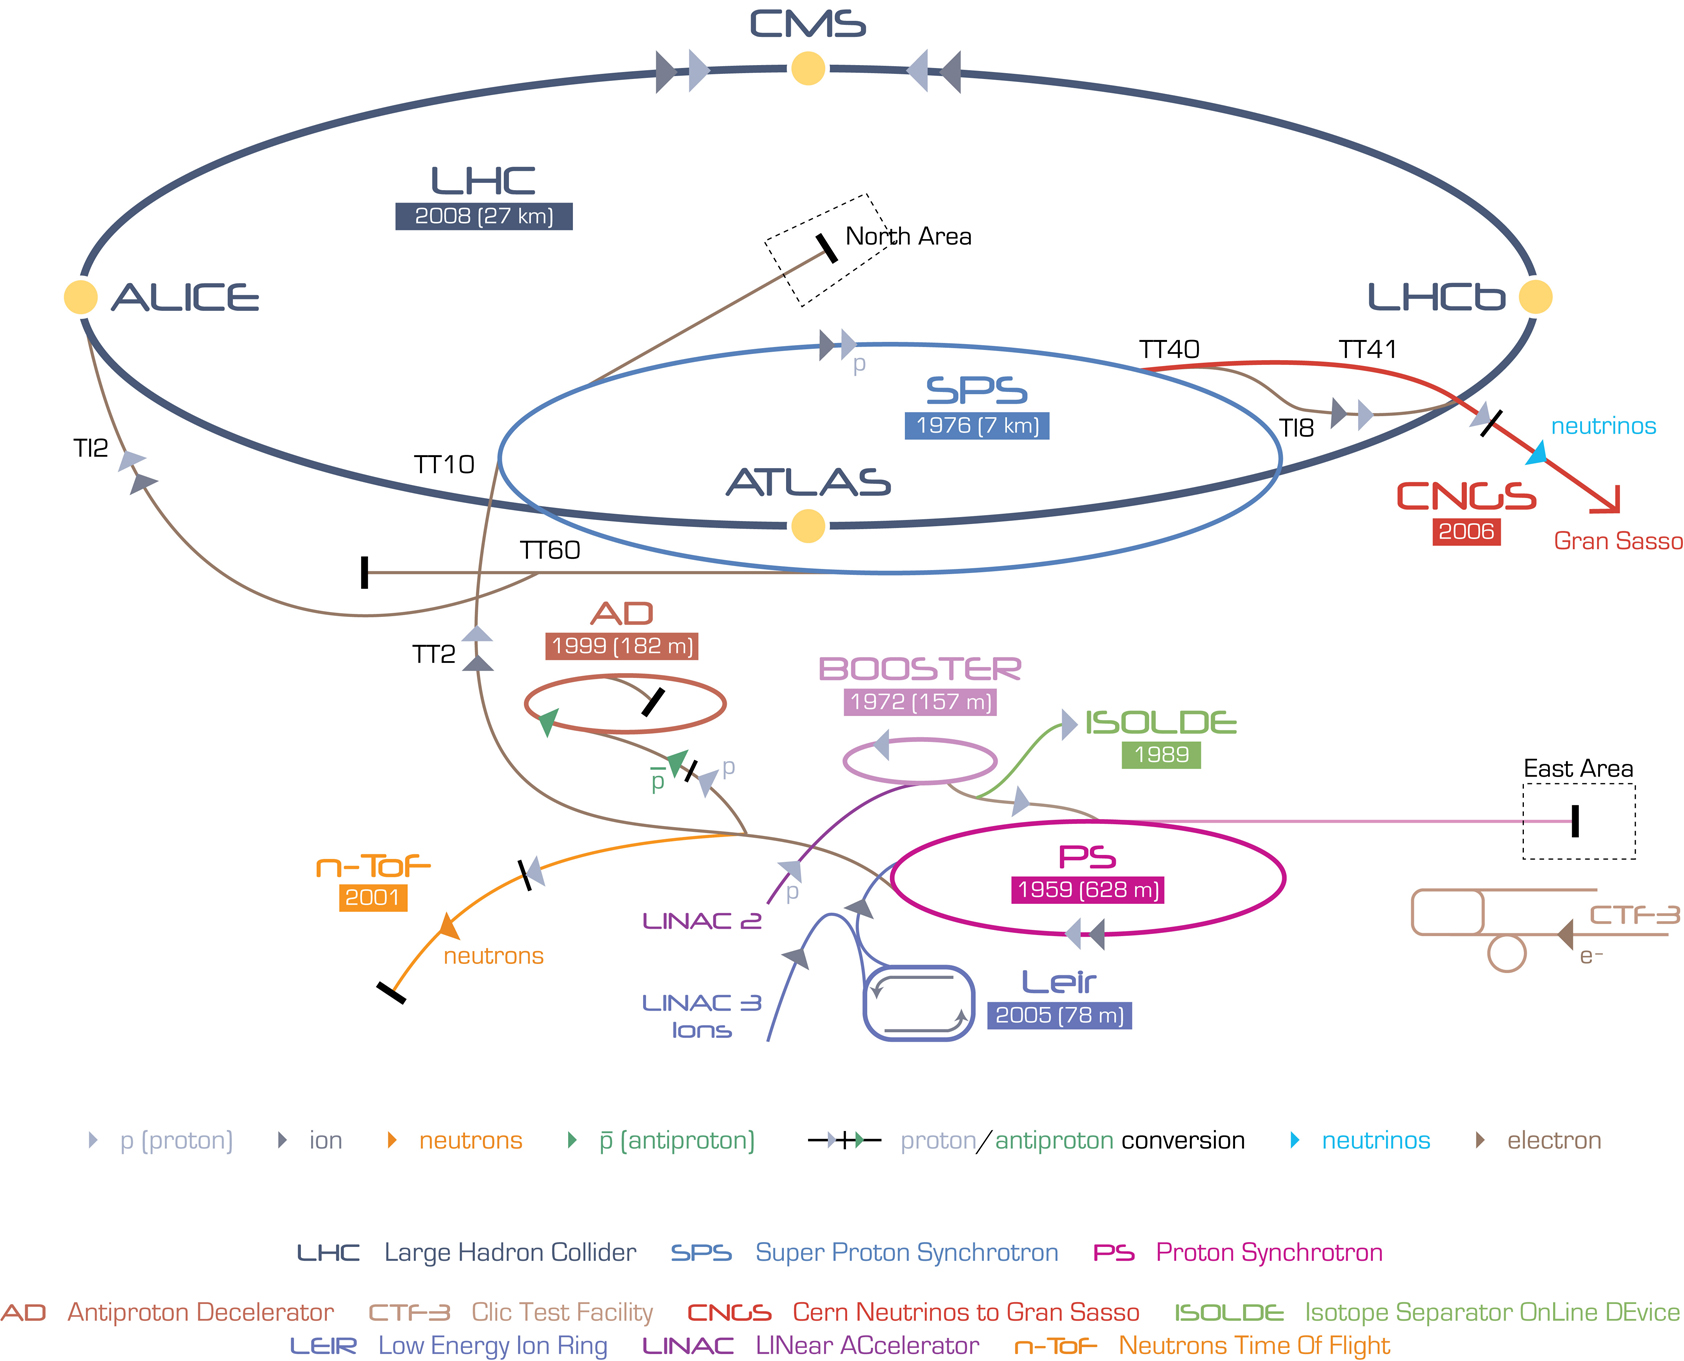
\includegraphics[width=0.95\textwidth]{PartDetector/Diagrams/Cern-Accelerator-Complex.jpg}
    \caption{The layout of CERN complex of experiments, note the main four LHC experiments located at different points around the ring.}
  \label{fig:DetectorLHCLayout}
\end{figure}

\section{The large hadron collider} \label{sec:the_large_hadron_collider}

The LHC accelerates two beams of protons in opposite directions and then collides them at the four interaction points (IPs) where the experiments are located. The protons come from hydrogen gas where the orbiting electron is removed by an electric field, leaving behind a bare proton. The beam acceleration occurs in several stages exploiting smaller experiments present at CERN. During 2010 and 2011 protons were accelerated to a beam energy of \SI{3.5}{\TeV}, creating a centre of mass energy of \SI{7}{\TeV} and then \SI{4}{\TeV} per beam in 2012 for a centre of mass energy of \SI{8}{\TeV}. Each beam is made of multiple bunches of protons, with as many as hundreds of billions of protons in each bunch. Bunches are grouped into \textit{bunch trains} with a designed \textit{bunch spacing} of \SI{25}{\ns} between each of the bunches that compose a single train. The bunch spacing and size of the bunch can be altered to adjust the amount of collisions and time between collisions. During 2011 a \SI{50}{\ns} bunch spacing was used to allow for early low luminosity analyses to be performed. The variation in the number of colliding bunches is shown in Figure~\ref{fig:DetectorBunchesColliding}.

\begin{figure}[htbp]
  \centering
    \begin{subfigure}[b]{0.95\textwidth}
      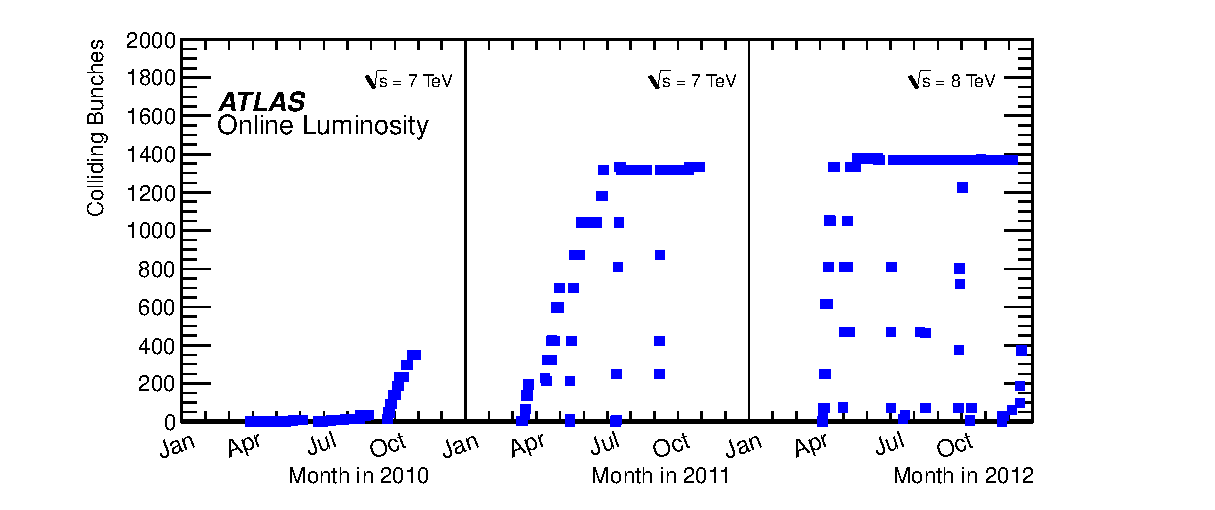
\includegraphics[width=\textwidth]{PartDetector/Plots/BunchesCollidingPerTime.eps}
      \caption{The number of bunches colliding per unit time at the LHC for the 2010, 2011 and 2012 $pp$ collision periods.}
      \label{fig:DetectorBunchesColliding}
    \end{subfigure}
  
    \begin{subfigure}[b]{0.95\textwidth}
      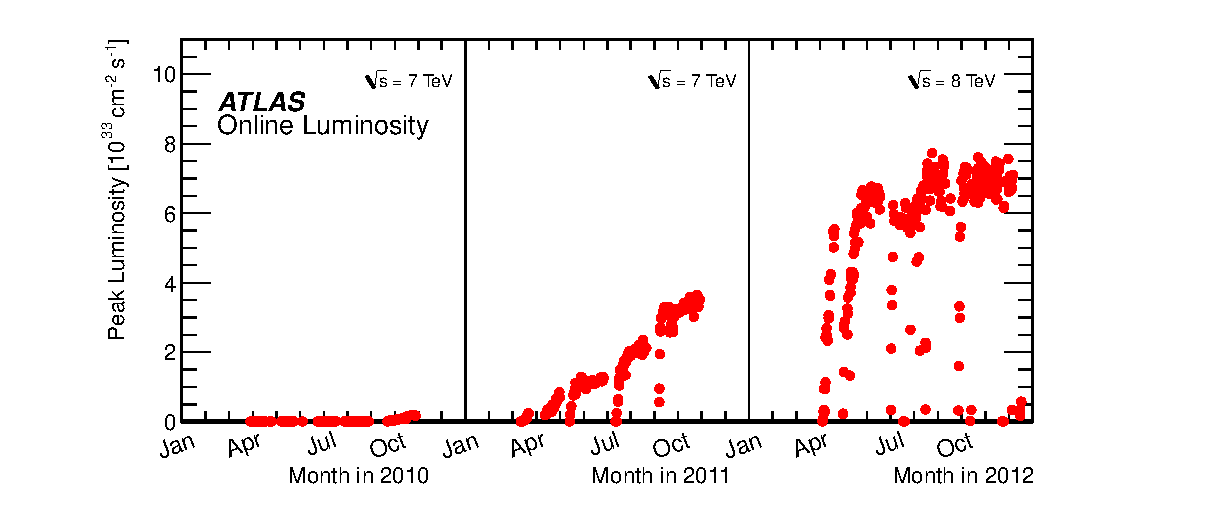
\includegraphics[width=\textwidth]{PartDetector/Plots/PeakLuminosityVsTime.eps}
      \caption{The peak luminosity per unit time at the LHC for the 2010, 2011 and 2012 $pp$ collision periods.}
      \label{fig:DetectorPeakLumi}
    \end{subfigure}
    \caption[Shown are the number of bunches colliding at the LHC and the peak luminosity per unit time.]{Shown are~\subref{fig:DetectorBunchesColliding} the number of bunches colliding at the LHC and~\subref{fig:DetectorPeakLumi} the peak luminosity per unit time~\cite{Detector:LuminosityResults}.}
  \label{fig:DetectorPerformance}
\end{figure}

The acceleration of the proton beams occurs in several stages in different accelerators. The beams are first accelerated in a linear collider (LINAC 2) to an energy of \SI{50}{\MeV} before being injected into the proton synchrotron booster (PSB). The beams are then boosted to \SI{1.4}{\GeV} by a varying magnetic field in the circular PSB. Beams are then passed into the proton synchrotron (PS) and then the super proton synchrotron (SPS) where the beam energy increases to \SI{26}{\GeV} and then \SI{450}{\GeV}. At this stage the beam is injected into the LHC and then accelerated to the final desired energy. The design energy is \SI{7}{\TeV} per beam for a total of \SI{14}{\GeV} centre of mass energy. The whole process can take a couple of hours, from the initial injection of the protons to stable beam conditions in the LHC.

As bunches overlap the protons that make up the bunches interact, the result of this interaction is known as an event. The number of events is proportional to the instantaneous luminosity $\Lagr$ of the collider. $\Lagr$ is a measure of the flux of particles per unit area per unit time can be defined as:

\begin{equation}
  \Lagr=fn_{b}\frac{N_1 N_2}{A}
\end{equation}
%
where $f$ is the frequency of revolution of the beam, $n_b$ the number of colliding pairs of bunches in the beam, $N_1$ and $N_2$ are the number of particles in each colliding bunch and $A$ is the cross section of the beam~\cite{Luminosity}. The peak luminosity evolution at the LHC is shown in Figure~\ref{fig:DetectorPeakLumi}.

The total amount of data collected is measured by the integrated luminosity $\Lagr_{\textrm{int}}$ defined as the time integral of $\Lagr$. Integrated luminosity has units of inverse area, usually expressed in terms of barns (\si{\barn})\footnote{\SI{1}{\per\barn}=\SI{e-28}{\per\square\meter}}. The probability for a given process to occur is expressed as the cross section $\sigma$ and the total number of events which proceed via said process is defined as:
%
\begin{equation}
  \sigma\int\Lagr \dd t
\end{equation}

The integrated luminosity delivered by the LHC and collected by the ATLAS detector in 2011 and 2012 is shown in Figure~\ref{fig:DetectorIntLumi}. The ATLAS detector does not record all data delivered by the LHC; approximately $6.5\%$ was not recorded.

\begin{figure}[htbp]
  \centering
    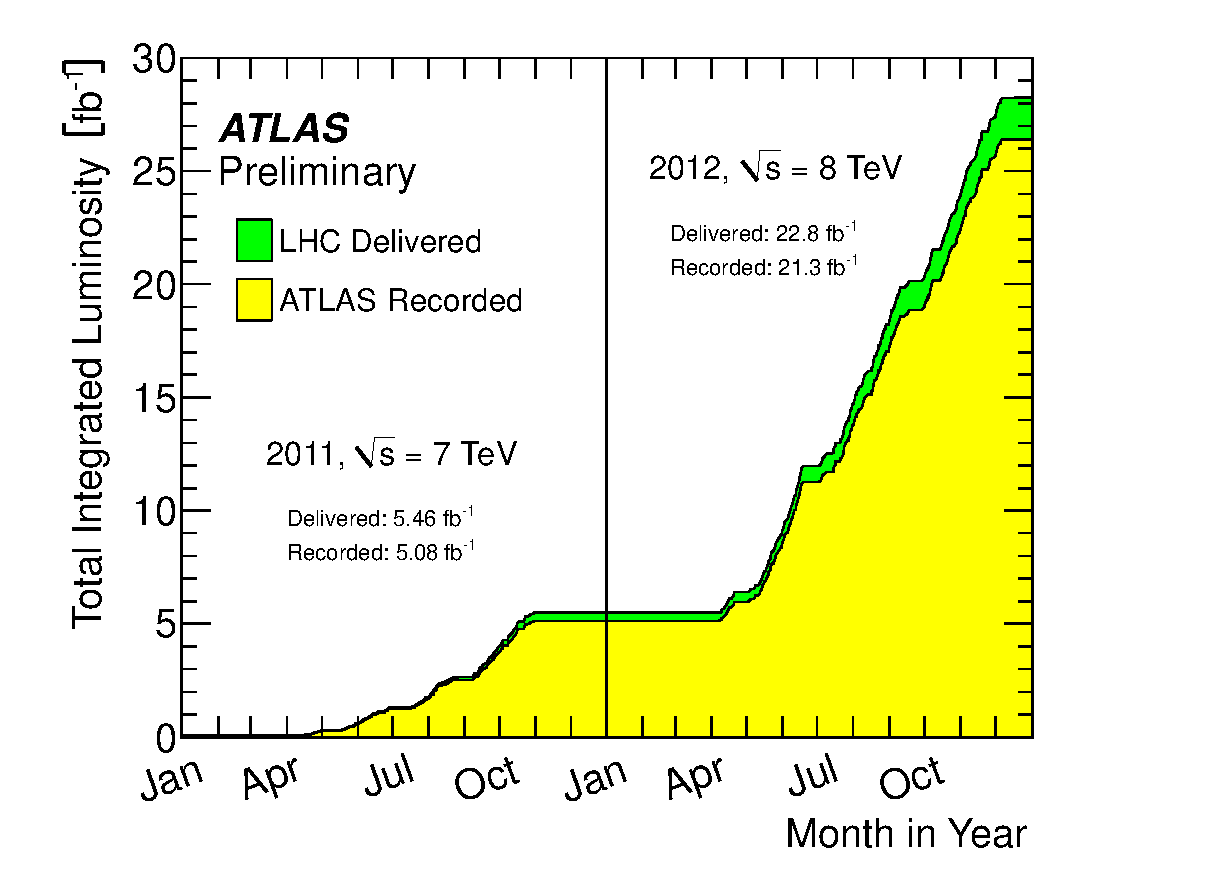
\includegraphics[width=0.70\textwidth]{PartDetector/Plots/IntegratedLuminosity20112012.eps}
    \caption[Distribution of the total integrated luminosity delivered by the LHC and the recorded by ATLAS for the 2011 and 2012 $pp$ collision period.]{Distribution of the total integrated luminosity delivered by the LHC and the recorded by ATLAS for the 2011 and 2012 $pp$ collision period~\cite{Detector:LuminosityResults,Luminosity}.} \label{fig:DetectorIntLumi}
\end{figure}

\subsection{Pile-up}

Due to the large number of interactions and the short time between collisions, multiple events can overlap into a single event. This has detrimental effects on physics analyses and is a determining factor in setting the instantaneous luminosity with which to perform data collection. This overlapping effect is collectively known as pile-up and is categorized into two types: in-time pile-up, where multiple $pp$ collisions occur during the same bunch crossing; and out-of-time pile-up, where the electric signals produced by previous collisions still remain to be read-out. This occurs when the time spacing between interactions is smaller than the read-out speed of the electronics. The number of interactions per crossing $\mu$ is shown in Figure~\ref{fig:DetectorBunchCrossingInteractions}, note that on average approximately thirty interactions occurred per bunch crossing in 2012. In comparison, in 2011 the average interactions per bunch crossing $\langle\mu\rangle$ varied from 5 in early 2011 to 15 at the end of the year.

\begin{figure}[htbp]
  \centering
    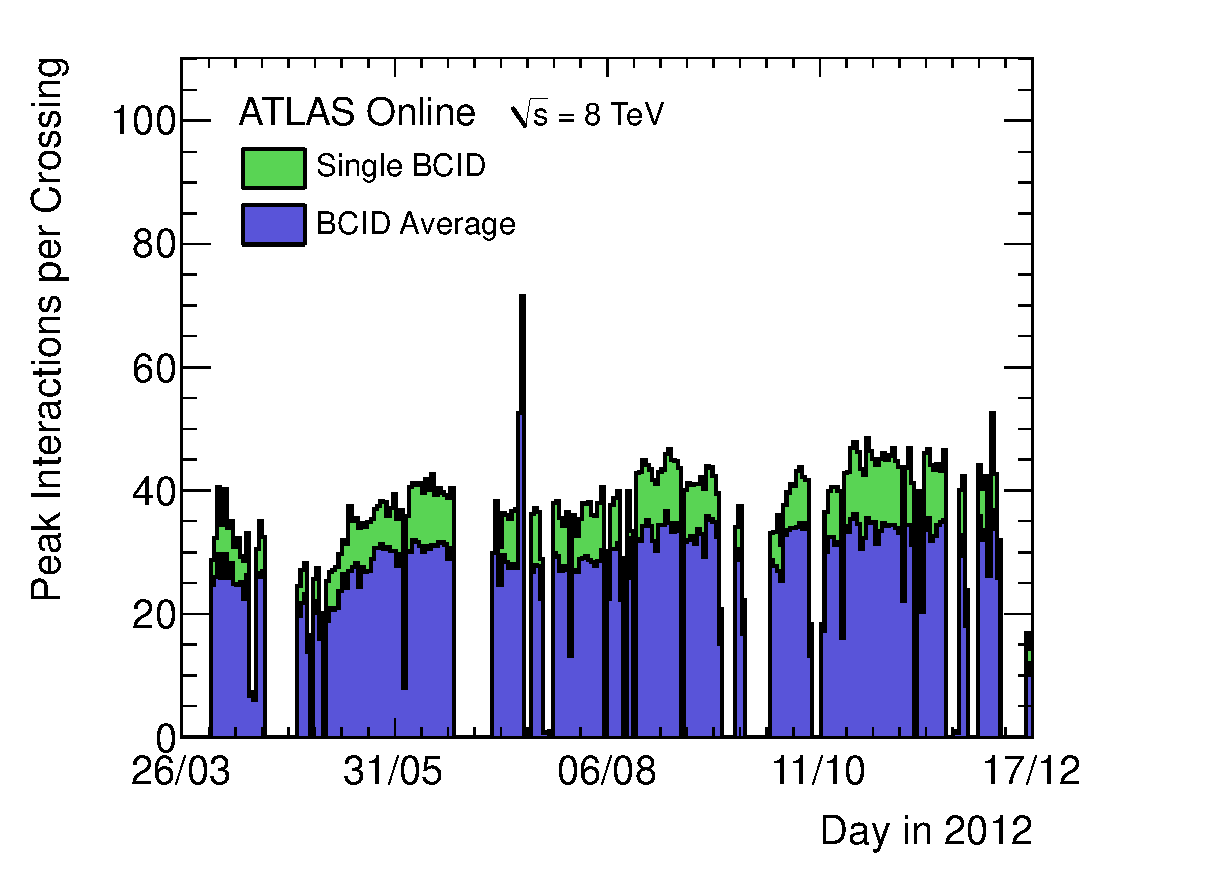
\includegraphics[width=0.70\textwidth]{PartDetector/Plots/peakBothMuByDay.eps}
    \caption[Number of interactions per bunch for the 2012 $pp$ data-taking period at ATLAS per day.]{Number of interactions per bunch crossing for the 2012 $pp$ data-taking period at ATLAS per day. Both the average number of interactions for all bunches and the maximum number of interactions are shown~\cite{Detector:LuminosityResults}.}
  \label{fig:DetectorBunchCrossingInteractions}
\end{figure}

\section{The ATLAS detector} \label{sec:the_atlas_detector}

The ATLAS~\cite{Detector:ATLASExperimentGeneral} experiment is a general-purpose detector which wraps around the IP providing large angular coverage. ATLAS is approximately cylindrical with a diameter of \SI{25}{\meter}, a total length of \SI{44}{\meter} and weighs \SI{7000}{\tonne}. The detector is made of several layers of instrumentation located at successively increasing radii as shown in Figure~\ref{fig:ATLASOverviewFigure}:

\begin{enumerate}
  \item \textbf{Inner Detector (ID)}: Located nearest to the beam-pipe and designed to measure the track of charged-particles.
  \item \textbf{EM Calorimeter}: Used for identification and measurement of electrons and photons.
  \item \textbf{Hadronic Calorimeter}: Used for the measurement of hadronic activity from hadronizing partons and missing transverse energy.
  \item \textbf{Muon Spectrometer (MS)}: The outermost detection layer, used for muon identification and measurement.
\end{enumerate}

Between these detection layers are magnets responsible for bending the path of the charged particles for the purpose of momentum measurement and particle identification. Triggering and data acquisition (TDAQ) systems also form part of the detector for the purposes of recording the data signals coming from the tracking and measurement systems. A brief description of these is provided in the coming sections. For a more detailed technical description of the detector and all subsystems see~\cite{Detector:ATLASExperimentGeneral}.

Lepton plus jets \ttbar\ events produce a final state that includes hadronic activity, electrons, muons and missing energy, so all elements of the detector are used in the reconstruction of such events. Additionally, the match \xsm\ tagger which is central to this thesis, relies on the reconstruction and fitting of ID tracks and MS tracks. A detailed description of this algorithm is provided in Section~\ref{sec:DetectorSTACO}.

\begin{figure}[htbp]
  \centering
    \includegraphics[width=0.90\textwidth]{PartDetector/Diagrams/ATLAS_Overall.eps}
    \caption[An overview diagram of the ATLAS experiment. Shown are all detection and tracking systems and the toroid magnet which encompasses them. Note also the muon system on the outside of the detector.]{An overview diagram of the ATLAS experiment. Shown are all detection and tracking systems and the toroid magnet which encompasses them. Note also the muon system on the outside of the detector~\cite{Detector:ATLASExperimentGeneral}.}
  \label{fig:ATLASOverviewFigure}
\end{figure}

A cylindrical coordinate system as used by all ATLAS publications has been adopted here. The coordinate system is constructed so that the $z$-axis is parallel to the beam axis. The $x$-axis is positive in the direction going from the IP to the centre of the LHC ring, and the positive $y$-axis points upwards. Thus the $x$-$y$ plane is transverse to the beam direction. All transverse variables such as the transverse momentum \pt, transverse energy \Et\ and missing transverse energy \met\ are measured along this plane. The distance perpendicular to the beam-pipe is denoted by $R$, the azimuthal angle $\phi$ is measured around the beam axis, and the polar angle $\theta$ is the angle from the beam axis. The pseudorapidity is defined as $\eta=-\ln\tan(\theta/2)$. The distance in the $\eta$-$\phi$ plane between two objects is denoted by $\Delta R$ and defined as $\Delta R = \sqrt{\Delta\eta^{2}+\Delta\phi^{2}}$. Finally side A of the detector is defined as the positive $z$ side and side C is the negative $z$.  The transverse impact parameter $d_{0}$ is defined as the distance of closest approach (perigee) of a track to the primary vertex (PV), and the longitudinal impact parameter $z_{0}$ is the distance in $z$ between the perigee and the primary vertex.

\subsection{Inner detector} \label{subsec:DetectorID}
The inner detector, shown in Figure~\ref{fig:DetectorIDOverview}, is a tracking detector located closest to the beam-pipe and used for momentum and impact parameter measurement, vertex and track reconstruction, and particle identification. The ID is designed to provide hermetic high-resolution tracking in the range $\aeta<2.5$.

\begin{figure}[htbp]
  \centering
    \includegraphics[width=0.85\textwidth]{PartDetector/Diagrams/ATLAS_ID.eps}
    \caption[Drawing of the ATLAS inner detector]{Drawing of the ATLAS inner detector~\cite{Detector:ATLASExperimentGeneral}.}
  \label{fig:DetectorIDOverview}
\end{figure}

The entire ID is contained within the central solenoid (CS) that generates a \SI{2}{\tesla} magnetic field for the purpose of momentum measurement. The trajectory of a charged particle is bent in the presence of a magnetic field by an amount proportional to the momentum of the particle
%
\begin{equation}
  r=\frac{\pt}{qB}
\end{equation}
%
where $r$ is the bending radius, \pt\ is the transverse momentum of the particle, $q$ is the charge of the particle, and $B$ is the magnetic field strength. Thus the momentum of the particle can be measured by reconstructing its trajectory through the detector. A particle with larger \pt\ would have a more straight trajectory than a particle with low \pt\ in the same magnetic field. For a central track with $\pt=\SI{5}{\GeV}$ the relative resolution on the measured transverse momentum is $\sim\SI{1.5}{\percent}$~\cite{Detector:ATLASExperimentGeneral}.

The reconstruction of interaction vertices is paramount, particularly when considering the large amount of pile-up observed at ATLAS. Interaction vertices are reconstructed by fitting all reconstructed tracks to a point. The primary vertex (PV) is then defined as the vertex with the largest amount of momentum associated with it. The reconstruction of secondary interaction vertices is used for the identification of short-lived particles such as $b$-hadrons and $\tau$.

\begin{figure}[htbp]
  \centering
  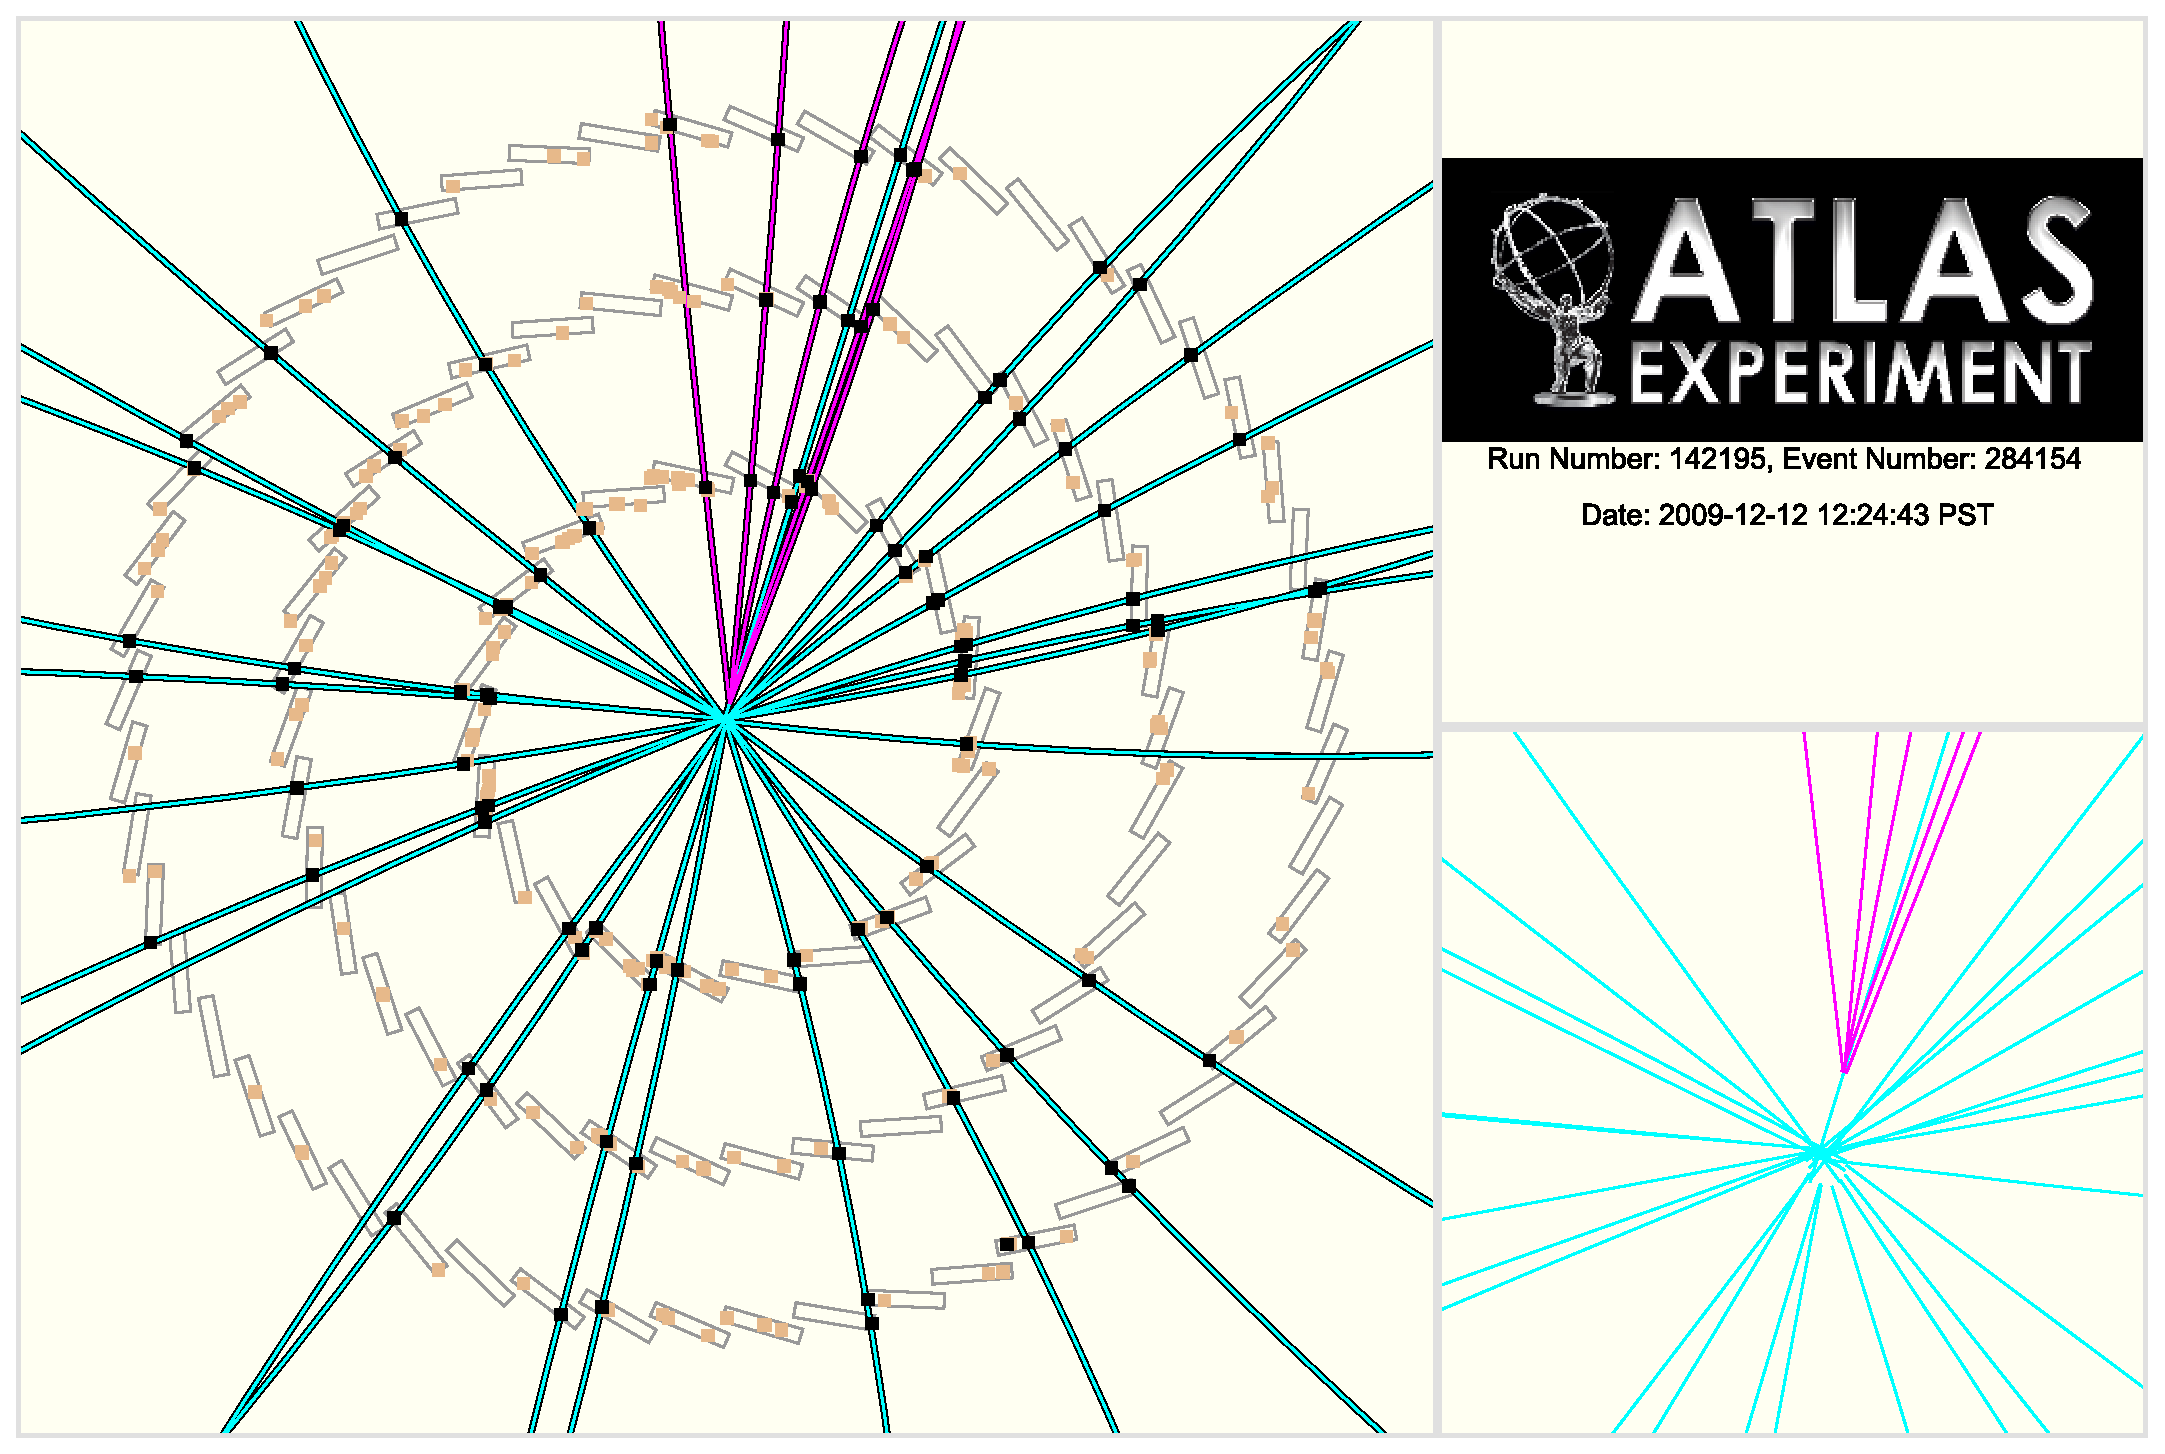
\includegraphics[width=0.75\textwidth]{PartDetector/Diagrams/fig_14.eps}
  \caption[An event display of an event as reconstructed by the ATLAS inner detector.]{An event display of an event as reconstructed by the ATLAS inner detector~\cite{Detector:ATLASExperimentGeneral}. Shown are the results of the vertexing algorithm where each line represents a track. the purple tracks have been fitted to a secondary vertex.}
  \label{fig:DetectorEventDisplayID}
\end{figure}

The ID is made of three separate tracking and detection systems located at increasing radii away from the beam-pipe, the full arrangement can be seen in Figure~\ref{fig:DetectorIDQuarter}, and a plane-view is shown in Figure~\ref{fig:DetectorIDTransverse}.

\begin{figure}
  \centering
    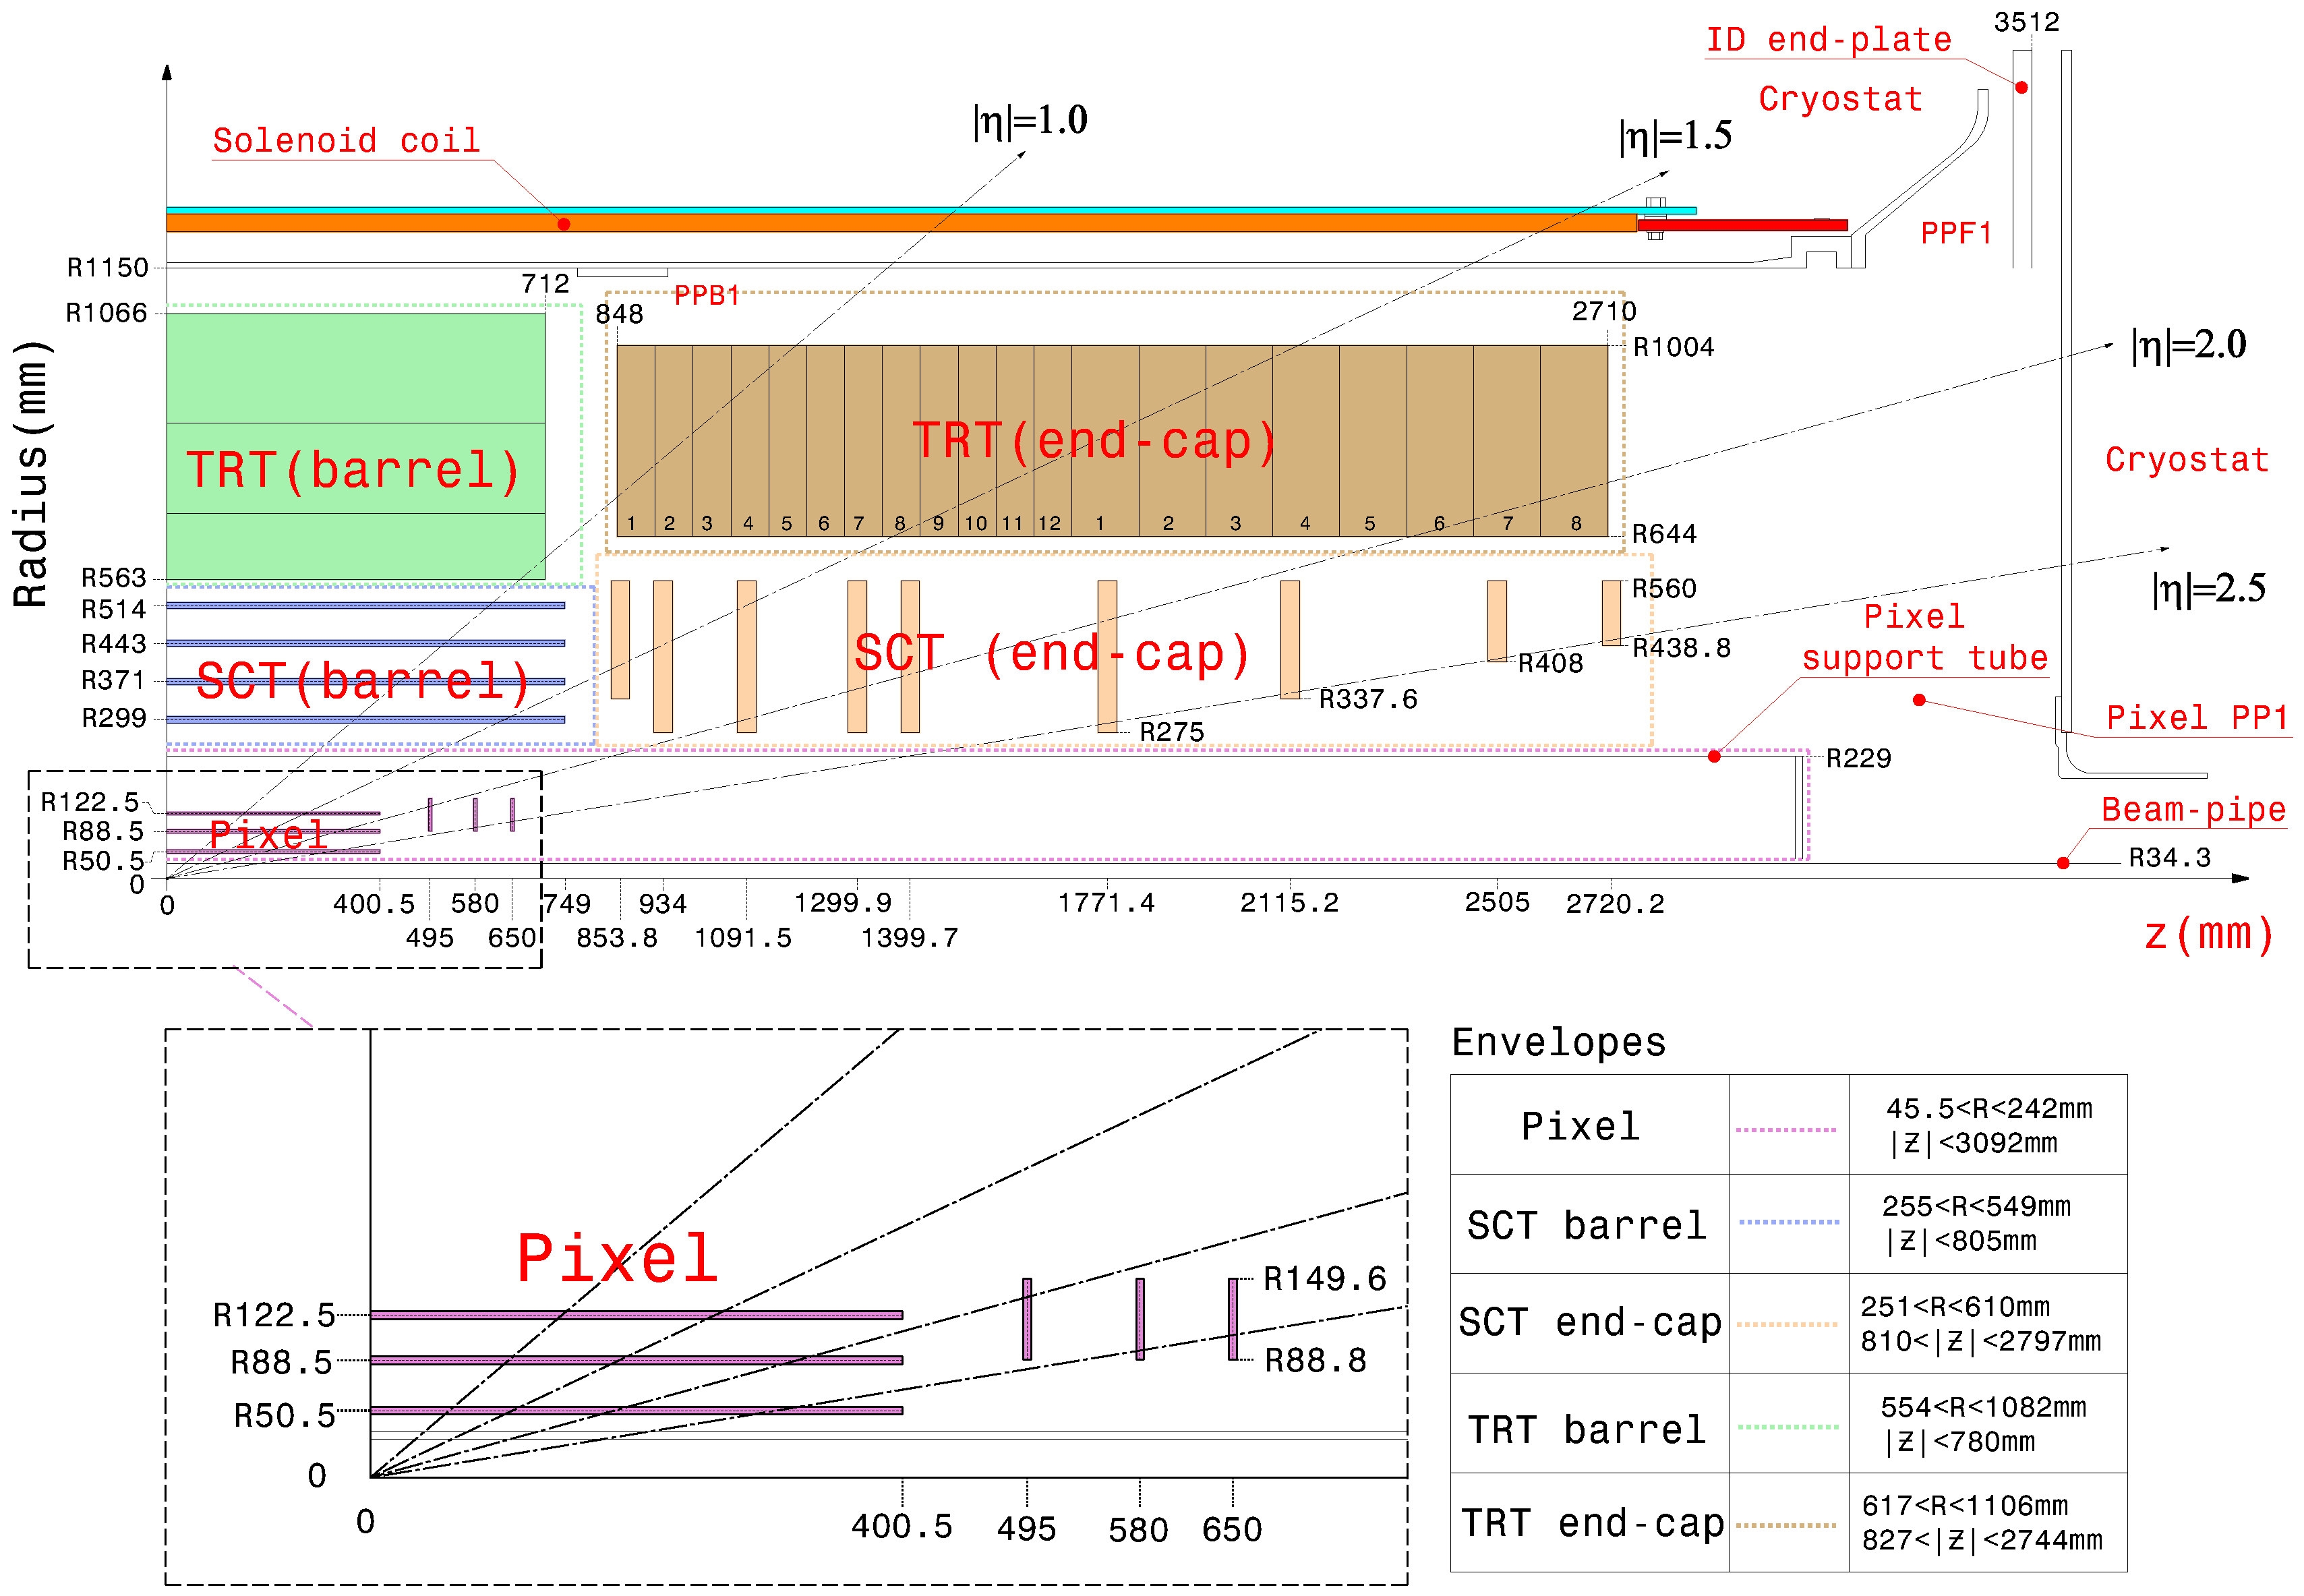
\includegraphics[width=0.75\textwidth]{PartDetector/Diagrams/Detector_ID_QuarterView.eps}
    \caption[Plan-view of a quarter-section of the ATLAS ID showing the major detector elements with its active dimensions and envelopes.]{Plan-view of a quarter-section of the ATLAS ID showing the major detector elements with its active dimensions and envelopes~\cite{Detector:ATLASExperimentGeneral}. Note also the $\eta$ markers showing the maximum coverage up to $\eta=2.5$.}
  \label{fig:DetectorIDQuarter}
\end{figure}
  
\begin{figure}
  \centering
    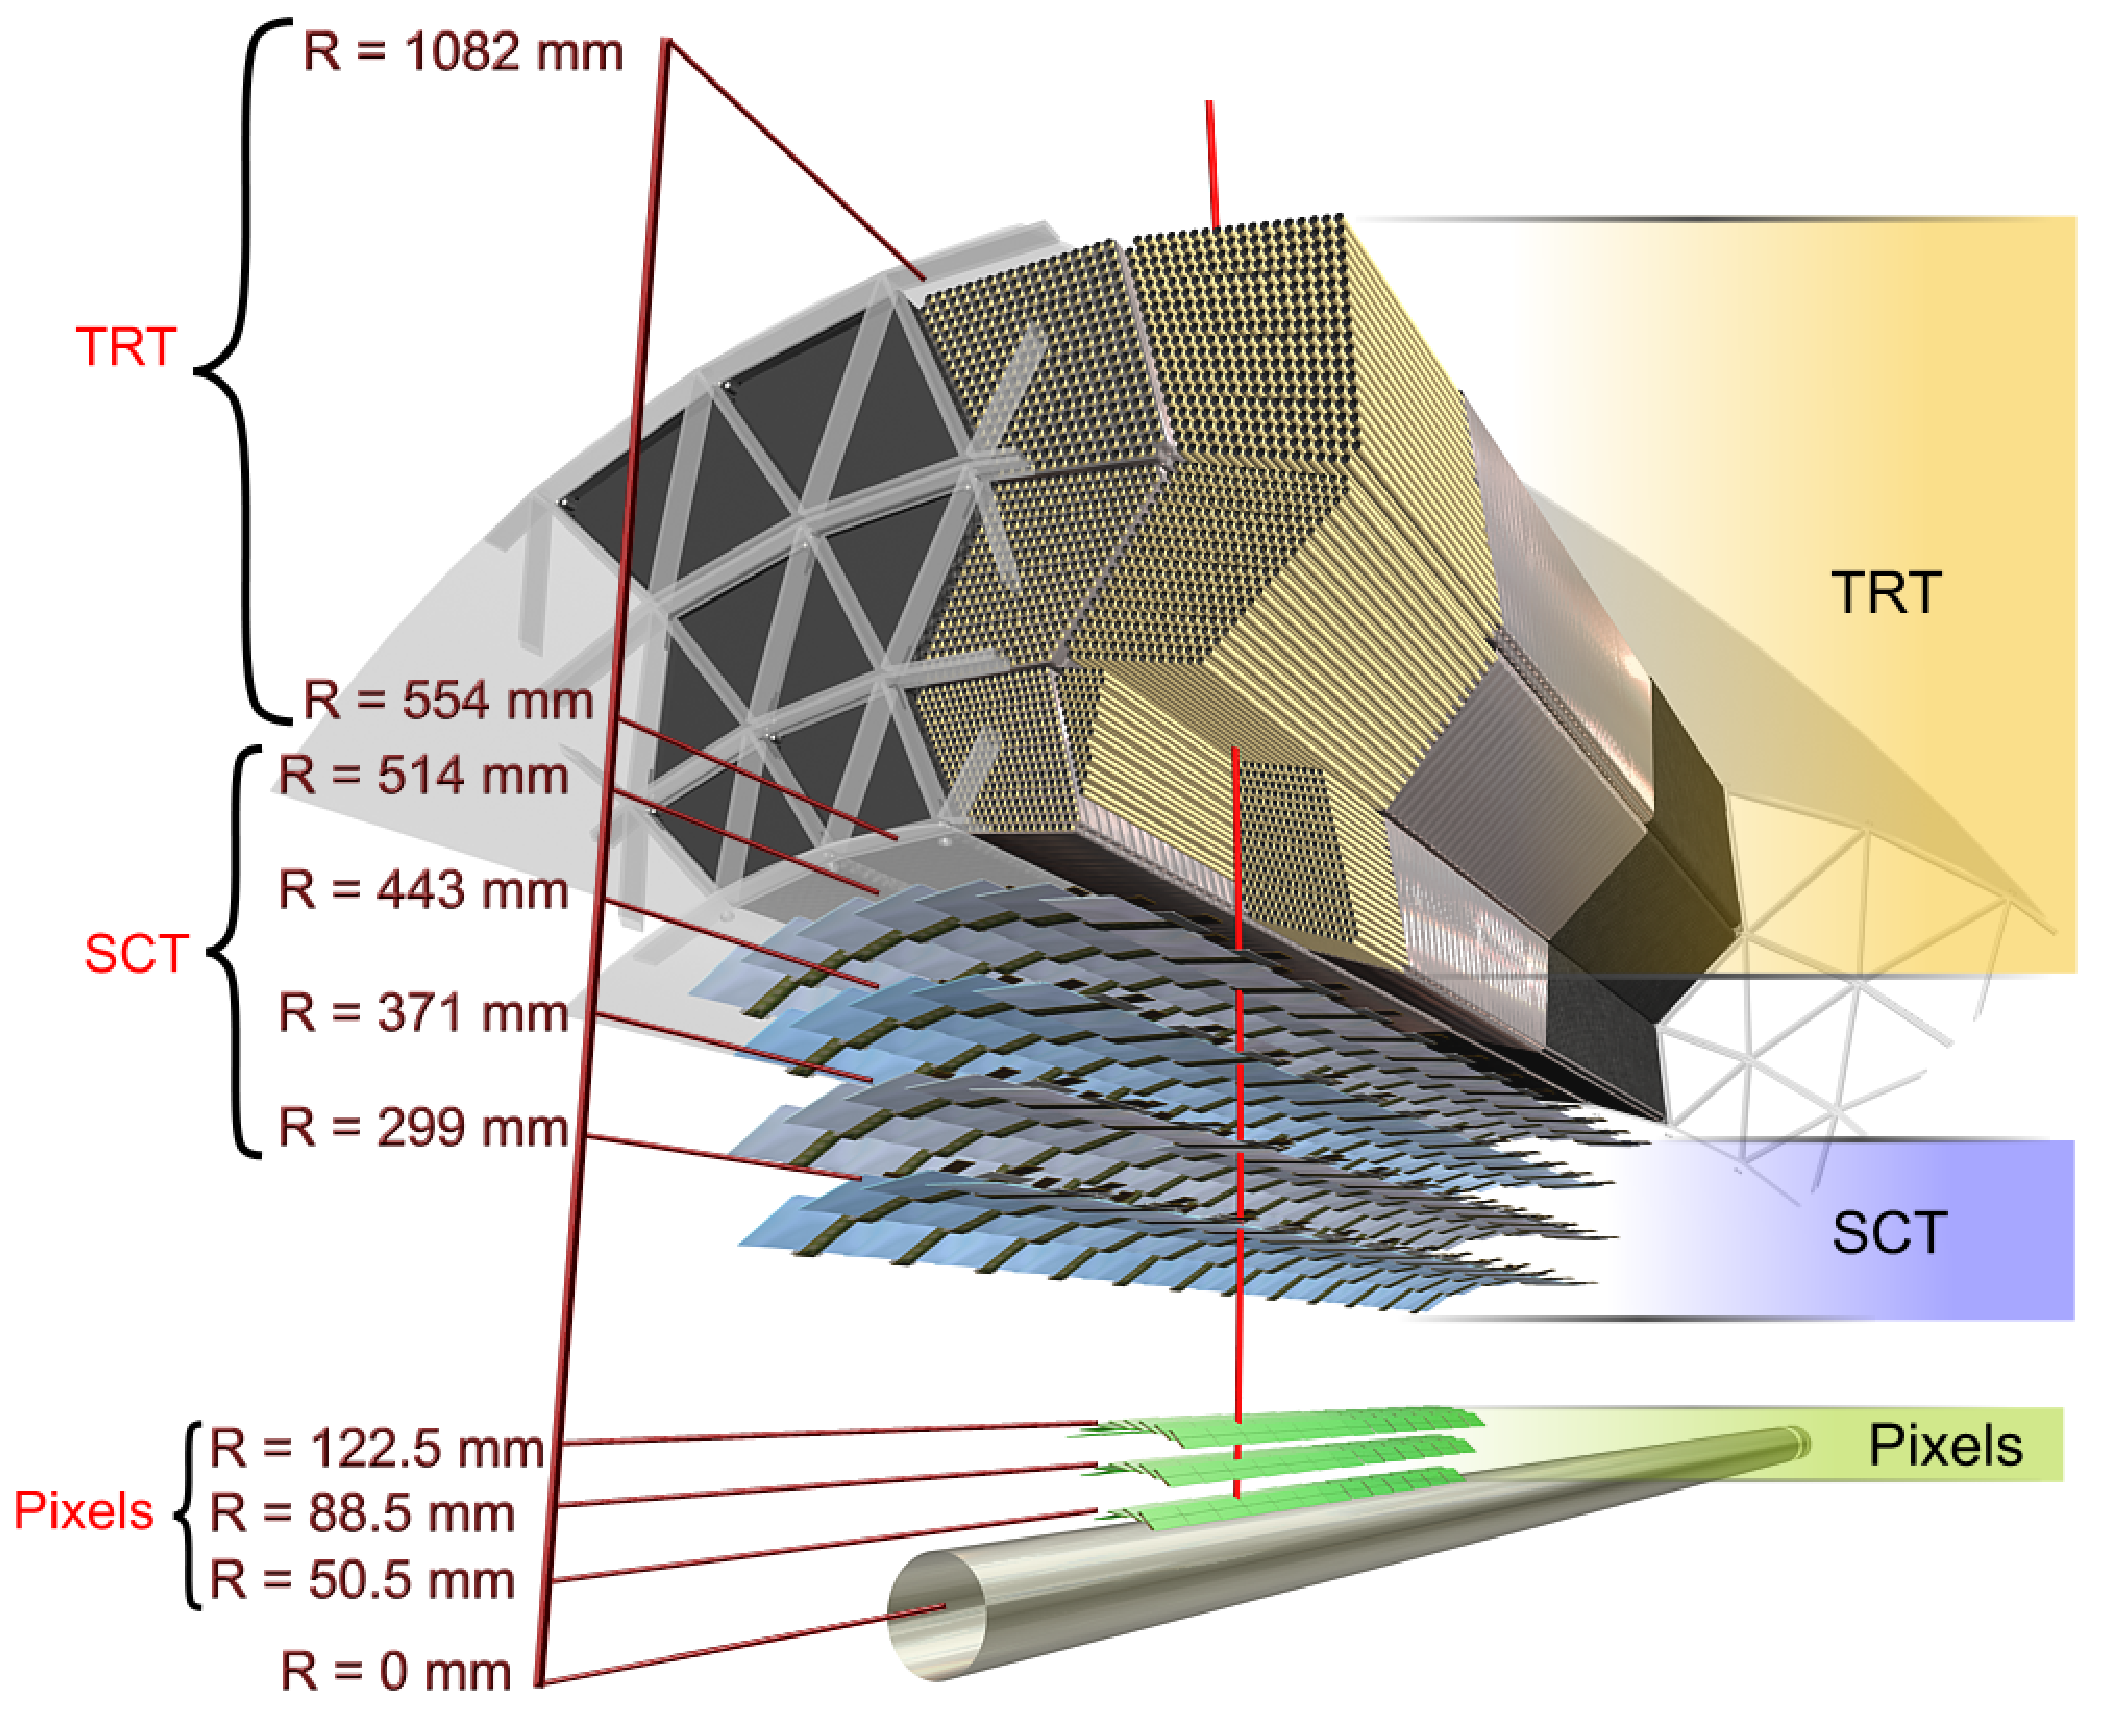
\includegraphics[width=0.75\textwidth]{PartDetector/Diagrams/ID_3D_Overview.eps}
    \caption[A drawing in the transverse plane of the ATLAS ID showing all major detection elements in the barrel regions.]{A drawing in the transverse plane of the ATLAS ID showing all major detection elements in the barrel regions~\cite{Detector:ATLASExperimentGeneral}. A charged particle track is shown traversing all the detector elements as a solid line.}
  \label{fig:DetectorIDTransverse}
\end{figure}

\subsubsection{Pixel detector}

The pixel detector is located nearest to the beam-pipe and provides high-granularity and precision for secondary vertex reconstruction. As a charged particle passes through a silicon pixel, several electron-hole pairs are created. The electrons and holes begin drifting in opposite directions under the influence of a voltage, and the charges are read out as a \emph{hit} through an electrode. The pixel detector consists of three silicon pixel sensor layers in the barrel region located at approximately \SIlist{5;9;12}{\cm} from the IP, and three disks at each side located at constant $R$ providing coverage up to $\aeta<2.5$. The barrel modules are overlapped in a turbine pattern to provide hermetic coverage. In the barrel region the modules provide an intrinsic resolution of \SI{10}{\um} in \rphi\ and \SI{115}{\um} in $z$~\cite{Detector:ATLASExperimentGeneral}. The disk sections have an intrinsic resolution of \SI{10}{\um} (\rphi) and \SI{115}{\um} ($R$).

\subsubsection{Semiconductor tracker}
The semiconductor tracker (SCT) located in the intermediate radius range is designed to provide eight hits per track contributing to the measurement of momentum, impact parameter, and vertex position. The SCT is made of four layers of stereo-pair silicon micro-strip sensors in the barrel region at increasing radii. The intrinsic resolutions are \SI{17}{\um} (\rphi) and \SI{580}{\um} ($z$). At the end-caps nine disks of silicon micro-strip modules provide large pseudorapidity coverage with a resolution of \SI{17}{\um} (\rphi) and \SI{580}{\um} ($R$)~\cite{Detector:ATLASExperimentGeneral}.

\subsubsection{Transition radiation tracker}
The transition radiation tracker (TRT) is the outermost tracking layer of the ID, and acts as both a tracker and transition radiation detector. Transition radiation (TR) is produced when a charged particle crosses the boundary between two materials with different dielectric constants. The probability of producing TR photons depends on the Lorentz factor of the particle $\gamma=E/m$. Thus for two particles of the same energy, a lighter particle will, on average, emit more ionization than a heavier particle.

The TRT is designed to provide up to \num{36} hits per track using straw-tube sensors. Each straw is \SI{4}{\mm} in diameter and is made of two \SI{35}{\micro\meter} thick Kapton multi-layer films bonded back-to-back. At the centre of each straw is a gold-plated tungsten wire with a diameter of \SI{31}{\micro\meter}. Each straw is filled with a mixture of gas (\SI{70}{\percent} Xenon, \SI{27}{\percent} $\textrm{CO}_{2}$ and \SI{3}{\percent} $\textrm{O}_2$). The tubes are surrounded by polypropylene-polyethylene fibres that act as radiators and allow for the production of TR, which later ionizes the gas mixture and is read-out through the gold-plated wire.

In the barrel, the \SI{144}{\cm} long straw-tubes are arranged in modules which contain between \num{329} and \num{793} straws. The end-cap disks are made of radially distributed \SI{36}{\cm} long straw-tubes. Each tube provides an intrinsic resolution of \SI{130}{\um} along its length~\cite{Detector:ATLASExperimentGeneral}. The combination of a large number of hits over a large radius allows measurements in the TRT to be made with an accuracy that can complement those made by the pixel detector.

\subsection{Calorimetry}
The ATLAS calorimeter is responsible for the measurement of the energy of particles that emerge from the event. Sampling calorimeters are used for this purpose, layers of absorber material (passive) are placed in the path of the particles forcing them to interact and shower. The amount of energy lost by the incident particle depends on the type of material the particle traverses, the energy of the particle, and the type of particle. At high energy, electrons lose energy predominantly via Bremsstrahlung, while the energy of photons is dissipated via pair production. The characteristic length associated with this energy loss is a material property known as the radiation length $X_0$.

For electrons, the energy as a function of material length traversed is
%
\begin{equation}
  E=E_0e^{-x/X_0}
\end{equation}
%
where $E_0$ is the initial energy, $x$ is the distance traversed, and $E$ is the energy of the particle at $x$. As an electron traverses one $X_0$ of material, its energy is reduced by a factor of $1/e$. For photons, the average number of photons traversing through a material length $x$ is reduced exponentially by a factor of $\frac{7}{9}X_0$. Thus the longitudinal length of the shower is proportional to the logarithm of the energy of the incoming particle.

The number of shower particles changes as a function of the hadronic interaction length $\lambda_{\textrm{int}}$ as
%
\begin{equation}
  N=N_{0}e^{-x/\lambda_{\textrm{int}}}
\end{equation}
%
where $N$ is the number of shower particles at length $x$ and $N_{0}$ is the initial number of incident particles. This is the characteristic length used when discussing the construction of the hadronic calorimeter. For a given material the $\lambda_{\textrm{int}}$ is much larger than $X_{0}$, therefore hadronic showers tend to be much broader and deeper than EM showers. Note that on average $1/3$ of the particle content of hadronic showers is electromagnetic, mostly due to pion decay into photons.

The energy of the resulting shower is measured by some sampling material (active) located behind the absorbers, this energy is proportional to the energy of the incident particle.

The type and thickness of material used is varied through the pseudorapidity range to improve energy measurement and reduce punch-through of particles into the muon system behind. Due to the intense radiation produced during collisions, radiation hardness is also an important factor in material choice.

The ATLAS calorimeter consists of the EM calorimeter, designed to measure photons and electrons covering $\aeta<3.2$; the hadronic calorimeter (HCal), which measures hadronic activity at $\aeta<3.2$; and the forward calorimeter (FCal) which provides energy measurement capability in at $3.1<\aeta<4.9$. As can be seen in Figure~\ref{fig:ATLASCalorimetryOverall}, the calorimetry envelopes the ID and CS providing hermetic coverage symmetric in $\phi$. This is particularly important for the measurement of \met\ resulting from weakly interacting particles escaping the detector.

\begin{figure}[htbp]
  \centering
  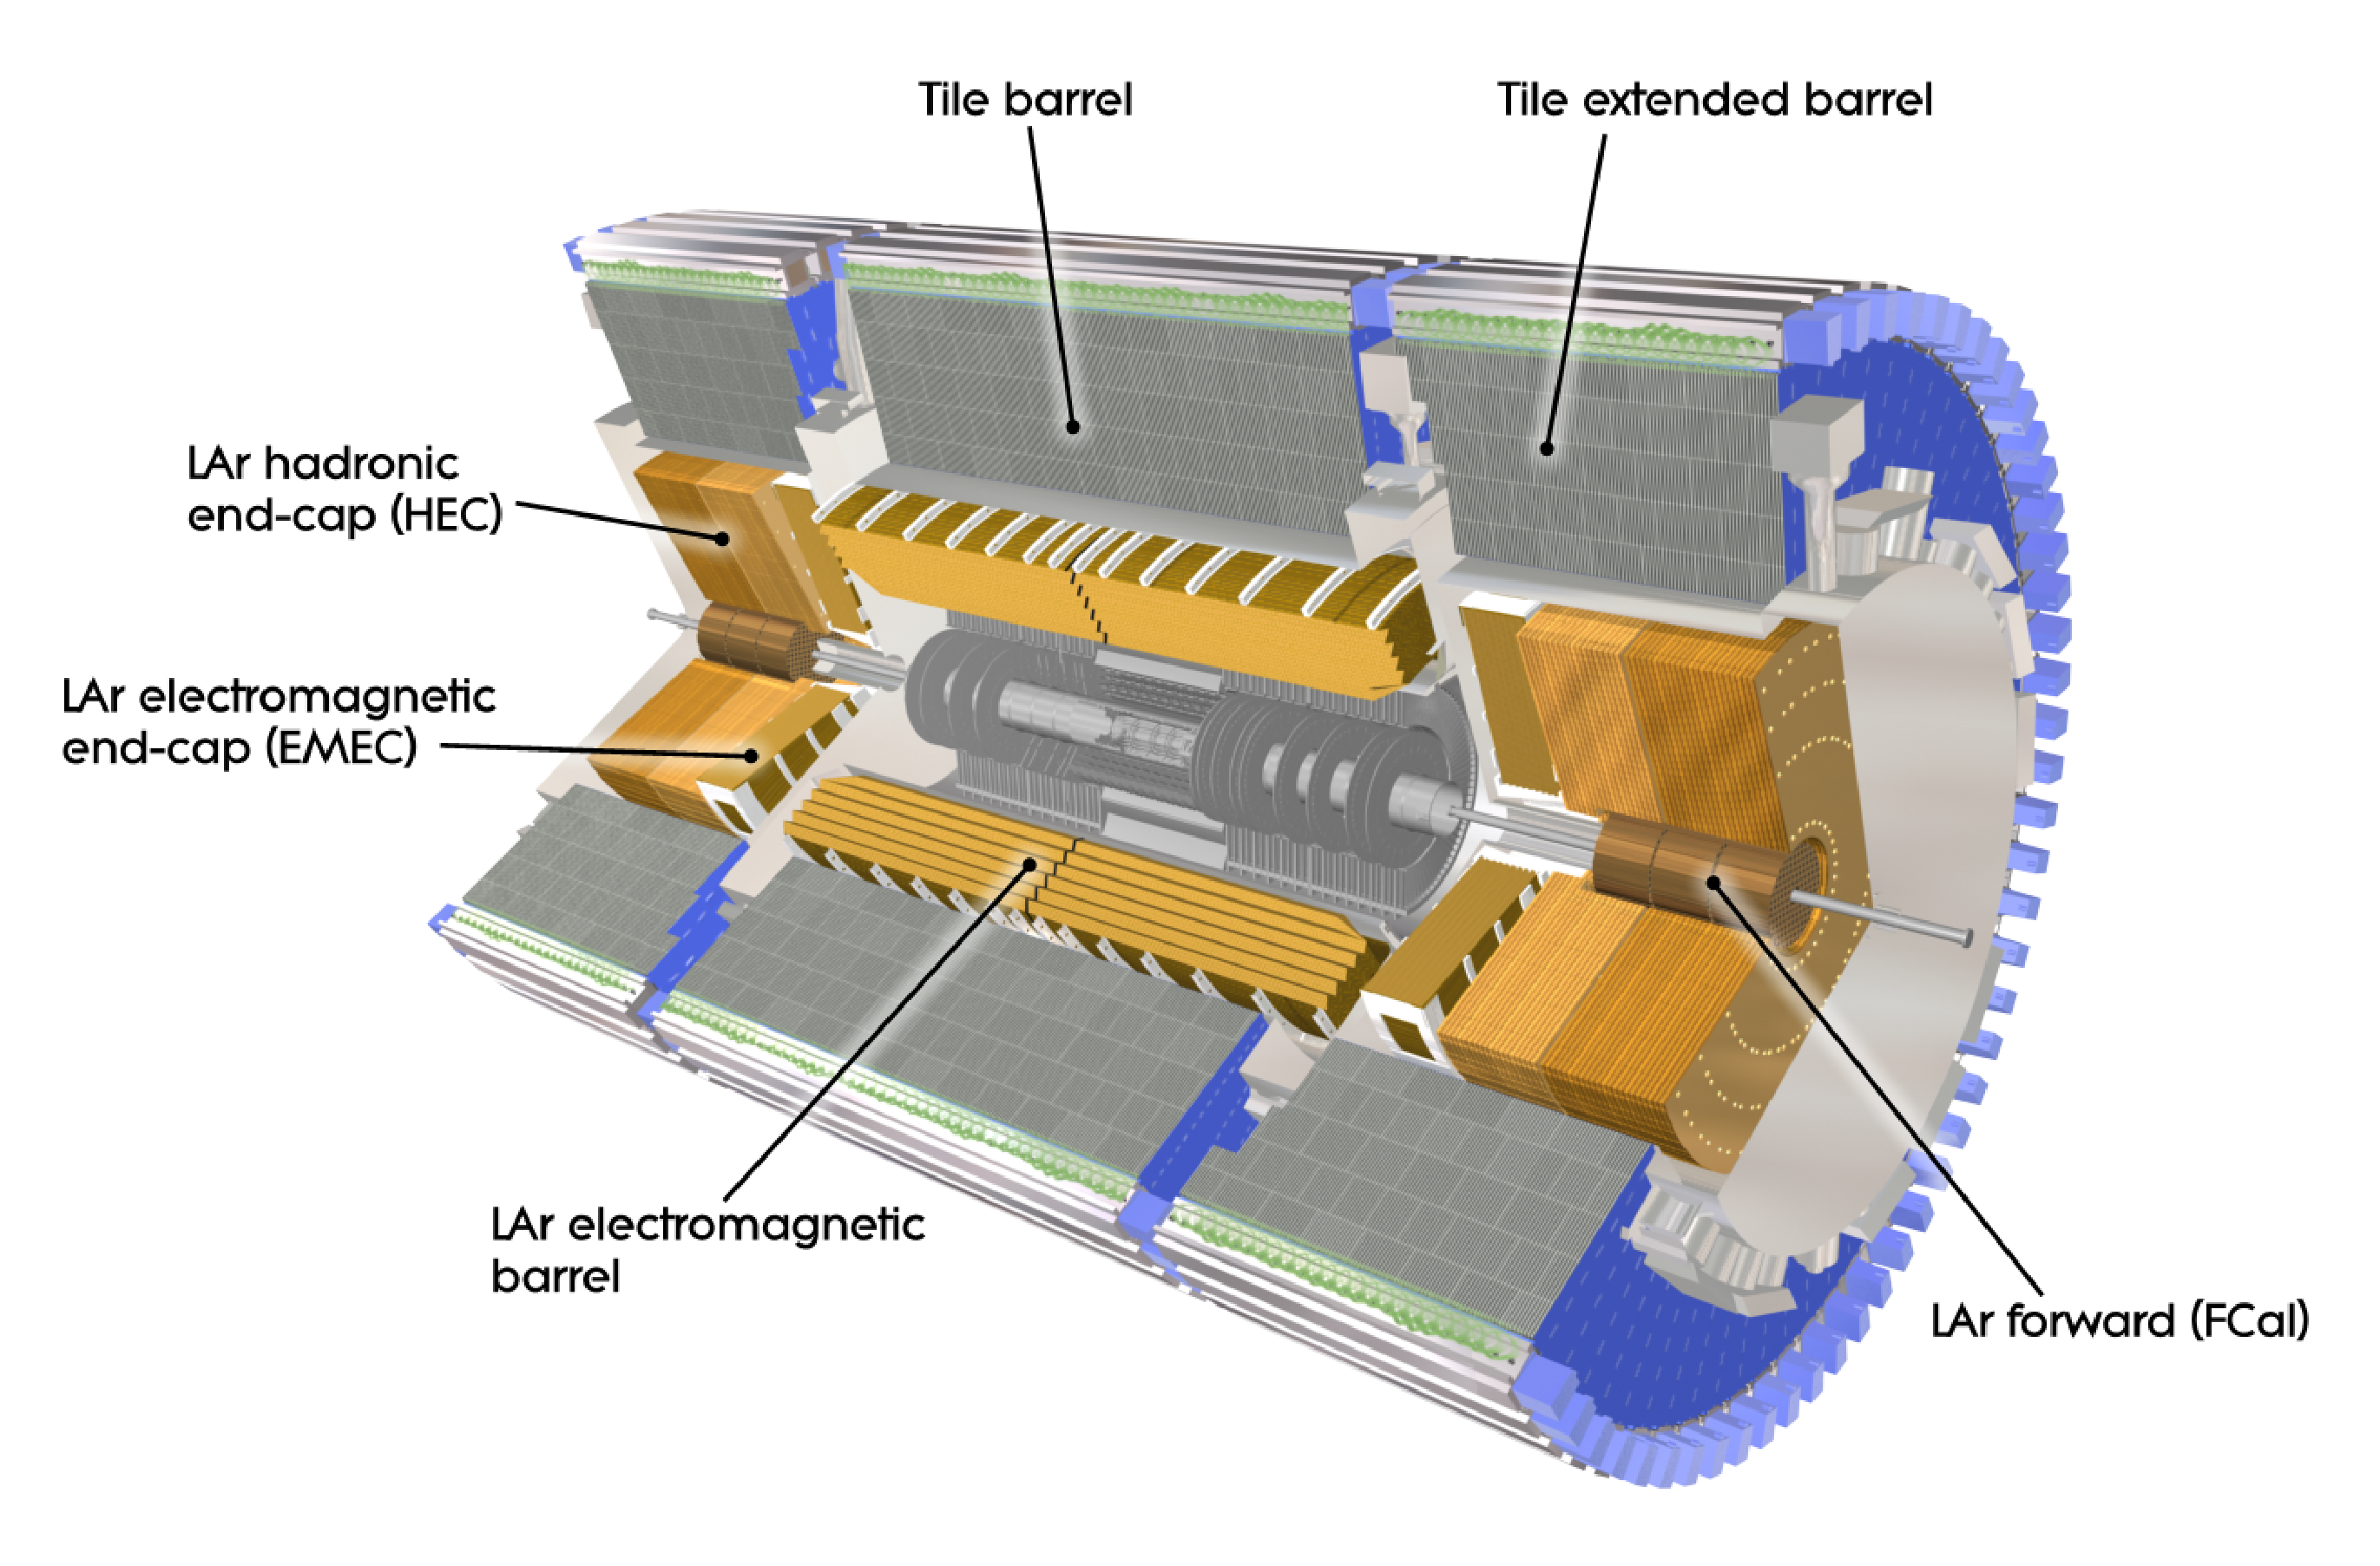
\includegraphics[width=0.90\textwidth]{PartDetector/Diagrams/ATLAS_Calorimetry.eps}
  \caption[A cut-away diagram of the ATLAS detector highlighting the calorimetry system.]{A cut-away diagram of the ATLAS detector highlighting the calorimetry system. Shown are the ECal barrel and end-cap, the HCal barrel and end-cap and the FCal end-cap~\cite{Detector:ATLASExperimentGeneral}.}
  \label{fig:ATLASCalorimetryOverall}
\end{figure}

\subsubsection{Electromagnetic calorimeter}
The EM calorimeter is made of a barrel section ($\aeta<1.475$) and two end-caps ($1.375<\aeta<3.2$). The barrel consists of two half-barrels separated by a \SI{4}{\mm} gap at $z=0$. The end-caps consist of two coaxial wheels, the outer ring covering $1.375<\aeta<2.5$ and the inner ring covering the range $2.5<\aeta<3.2$. The pseudorapidity region $1.37<\aeta<1.52$, known as the ``crack'' region, is not used for precision physics due to the large amount of material between the interaction point and the calorimeter.

The EM calorimeter employs liquid argon (LAr) as the active material due to its intrinsic radiation hardness and response over time, and lead as the passive material arranged in an accordion geometry for full $\phi$ symmetry. Particles interact with the lead absorbers creating a shower which ionizes the layers of LAr. A potential is applied across the LAr material allowing for signal read-out via Kapton/copper electrodes. The total thickness of the EM calorimeter is $>24X_{0}$ in the barrel and $>26X_{0}$ in the end-caps. The amount of material is optimized in pseudorapidity to enhance energy resolution. The amount of material, measured in terms of $X_{0}$, before and in the EM calorimeter is shown in Figure~\ref{fig:DetectorInteraction}.

\begin{figure}[htbp]
  \centering
  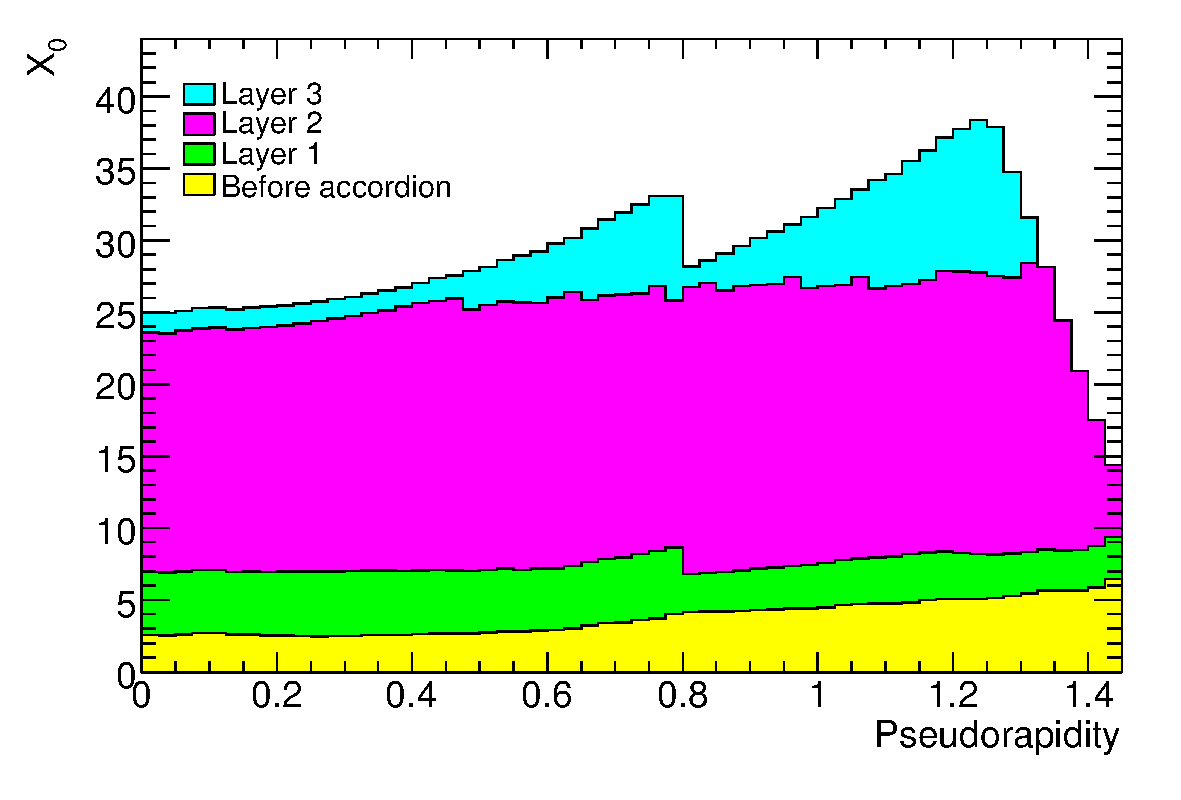
\includegraphics[width=0.46\textwidth]{PartDetector/Plots/x0_layers_barrel_csc03.pdf}
  ~
  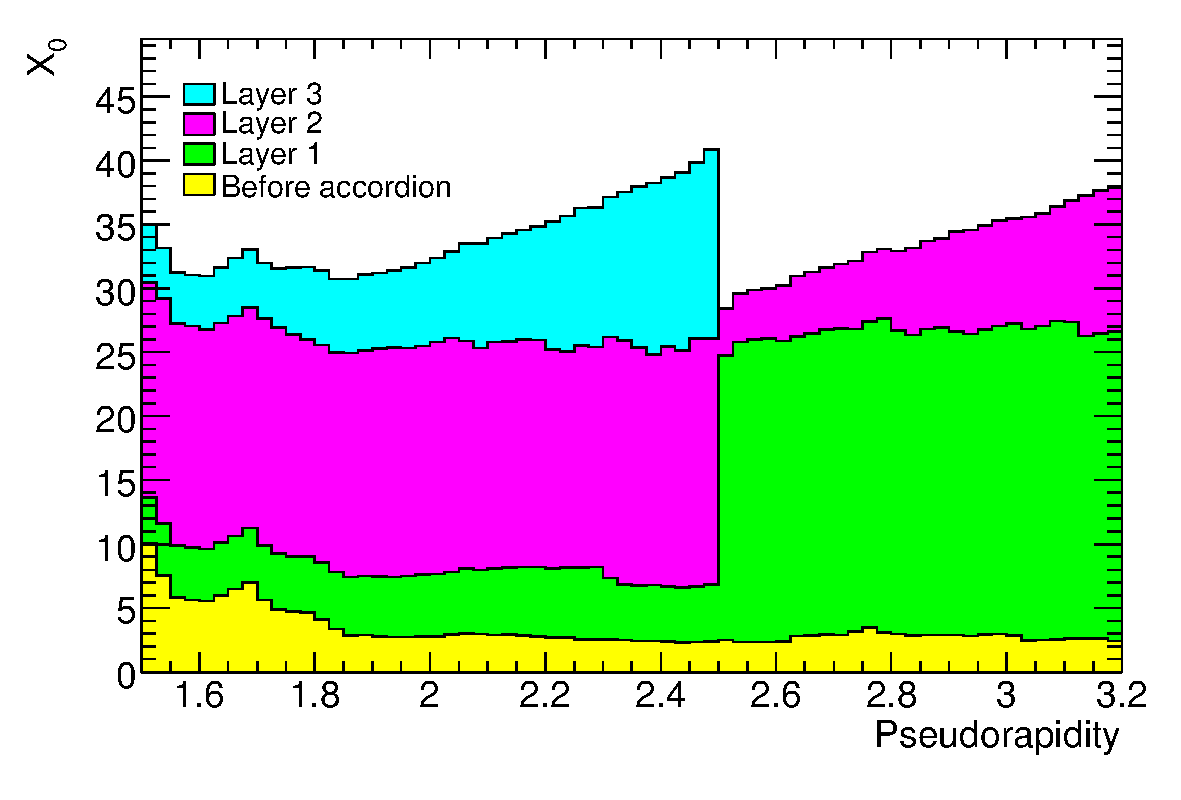
\includegraphics[width=0.46\textwidth]{PartDetector/Plots/x0_layers_endcap_csc03.pdf}
  \caption[Cumulative amounts of material, in units of radiation length $X_{0}$, as a function of $|\eta|$ in front and in the EM calorimeter at the ATLAS detector.]{Cumulative amounts of material, in units of radiation length $X_{0}$, as a function of $|\eta|$ in front and in the EM calorimeter at the ATLAS detector~\cite{Detector:ExpectedPerf}. The left-hand plot shows the amount of material in the barrel region and the right-hand plot shows the material in the endcap region.}
  \label{fig:DetectorInteraction}
\end{figure}

In the region devoted to precision physics the EM calorimeter is divided into three segments as shown in Figure~\ref{fig:DetectorECalSegment}, the strip layer is designed to improve particle identification and pseudorapidity measurement. The design energy resolution for all components of the calorimeter are shown in Table~\ref{tab:DetectorCaloResolution}.

\begin{table}[htb]
  \ra{1.3}
  \centering
  \begin{tabular}{@{}ll@{}}
    \toprule
    Section   & Resolution \\
    \midrule
    EM Barrel & $\frac{10\%}{\sqrt{E}}\oplus0.7\%$ \\
    EMEC      & $\frac{10\%}{\sqrt{E}}\oplus0.7\%$ \\
    HEC       & $\frac{100\%}{\sqrt{E}}\oplus10\%$ \\
    FCAL      & $\frac{100\%}{\sqrt{E}}\oplus10\%$ \\
    % EM Barrel & $\frac{10.1\%}{\sqrt{E}}\oplus0.17\%$~\cite{Energy} \\
    % HEC       & $\frac{70.6\%}{\sqrt{E}}\oplus5.8\%$ \\ MEASURED
    % FCAL      & $\frac{95\%}{\sqrt{E}}\oplus7.5\%$~\cite{Detector:FCalMeasuredPerf} \\ MEASURED
    \bottomrule
  \end{tabular}
  \caption[Design energy resolution of all ATLAS calorimeter components.]{Design energy resolution of all ATLAS calorimeter components~\cite{Detector:ATLASExperimentGeneral}. The resolution is made of a sampling term ($\nicefrac{1}{\sqrt{E}}$) associated with the choice of passive and active materials and the construction of the layers, and a constant term associated with the depth of the detector, cracks and dead material.} \label{tab:DetectorCaloResolution}
\end{table}

\begin{figure}[htbp]
   \centering
   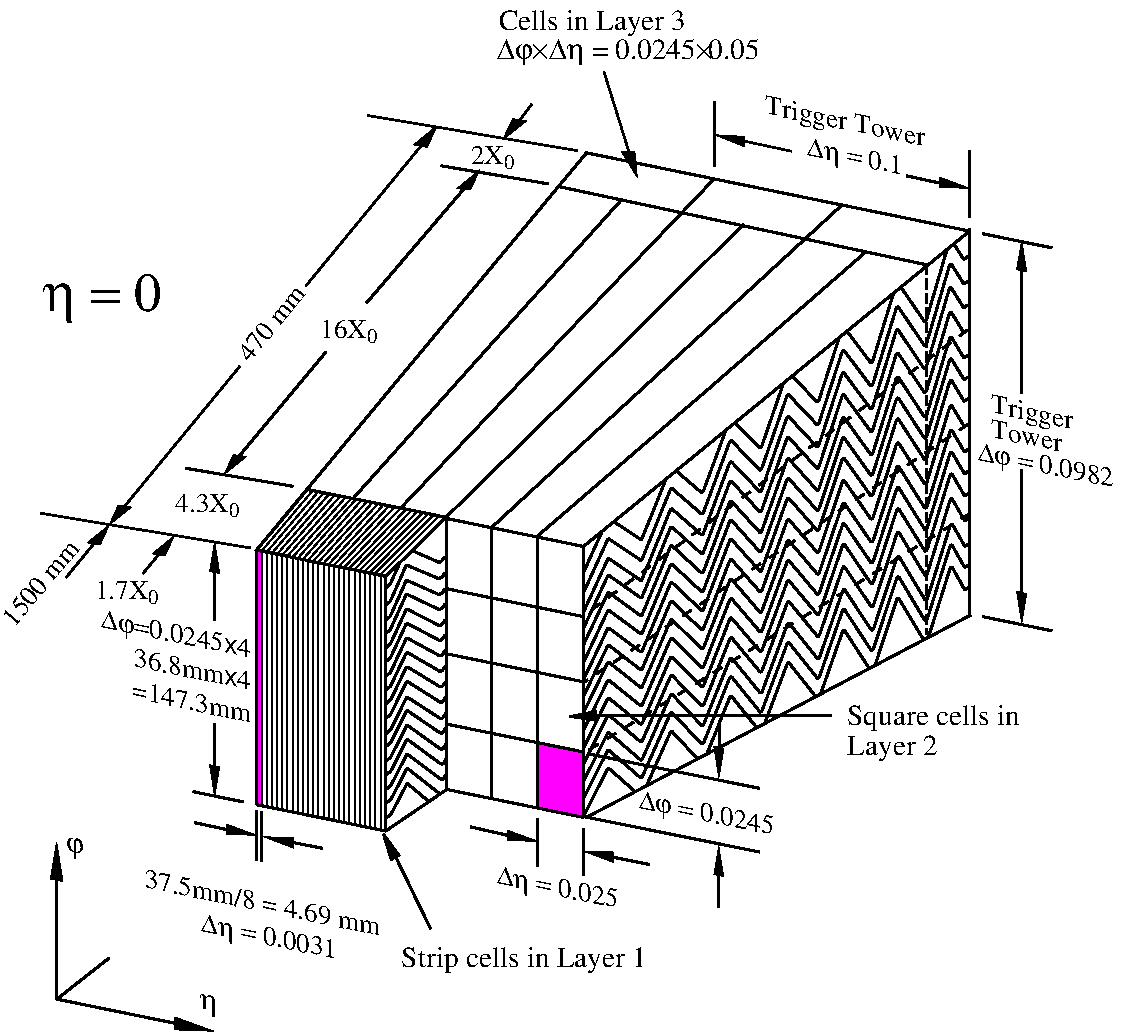
\includegraphics[width=0.75\textwidth]{PartDetector/Diagrams/LARG3-TDR-barrelM.pdf}
   \caption[Cut-away diagram of the EM calorimeter barrel at $\eta=0$.]{Cut-away diagram of the EM calorimeter barrel at $\eta=0$~\cite{Detector:ATLASExperimentGeneral}. Shown are the three different layers with varying cell structures. The strip section is designed to enhance particle identification and position measurement in $\eta$.}
   \label{fig:DetectorECalSegment}
 \end{figure} 

\subsubsection{Hadronic calorimeter}
The hadronic calorimeter uses different types of passive and active material to accommodate for the varying conditions in different regions of the detector. The structure of the detector and the materials used must provide good energy resolution, full symmetric coverage for the purpose of \met\ measurement, full containment of all hadronic activity to prevent punch-through to the muon system, and be sufficiently radiation hard. The hadronic calorimeter consists of two parts: a scintillator tile calorimeter in the barrel region and a LAr calorimeter in the end-cap.

The tile calorimeter is located directly outside the EM calorimeter. The barrel portion covers $\aeta<1.0$ and the two extended barrels cover the range $0.8<\aeta<1.7$. The tile calorimeter uses steel as the passive material and scintillating tiles as the active material. The resulting hadronic showers enter the scintillating tiles and produce photons which are passed to photomultiplier tubes. The total detector thickness which is tile-instrumented is $9.7\lambda_{\textrm{int}}$ at $\eta=0$.

The hadronic end-cap (HEC) uses LAr technology due to its radiation-hardness in this challenging high pseudorapidity region. The HEC consists of two independent wheels per end-cap covering the range $1.5<\aeta<3.2$ overlapping the tile calorimeter at low pseudorapidity and the forward calorimeter located at high pseudorapidity.

\subsubsection{Forward calorimeter}

The forward calorimeter (FCal) is responsible for energy measurement in the very high pseudorapidity range $3.1<\aeta<4.9$ of both electromagnetic and hadronic activity. Due to the large amount of radiation in this region, LAr is employed as the active material. The FCal consists of three layers: the first made primarily of copper, designed mostly for the measurement of electromagnetic activity, while the two outer tungsten layers are responsible for hadronic activity measurement.

\subsection{Muon spectrometer}

The muon spectrometer is the outermost layer of the ATLAS detector (Figure~\ref{fig:DetectorDrawingMuonSystem}) and is responsible for the precision measurement of \pt\ of charged-particles that pass-through the ATLAS calorimetry. It is designed to have a precision of \SI{10}{\percent} at a momentum of \SI{1}{\TeV}~\cite{Detector:ATLASExperimentGeneral}. Muon tracking performance is vital to the SMT tagger described in Section~\ref{sec:DetectorSLT}, as it relies on the precise reconstruction of muon tracks in the ID and MS.

Due to their larger mass, muons tend to have a larger transverse momentum and do not lose as much energy through photon emission. As a result, muons tend to traverse the hadronic calorimeter and escape the detector volume. The muon system provides measurement of these particles up to $\aeta<2.7$ and triggering up to $\aeta<2.4$. Measurement of \pt\ is facilitated by the magnetic field generated by the large toroid magnet in the barrel region $\aeta<1.4$ and two smaller end-cap magnets in $1.6<\aeta<2.7$. In the transition region at $1.4<\aeta<1.6$, deflection is provided by both barrel and end-cap fields. 

\begin{figure}[p]
  \centering  
  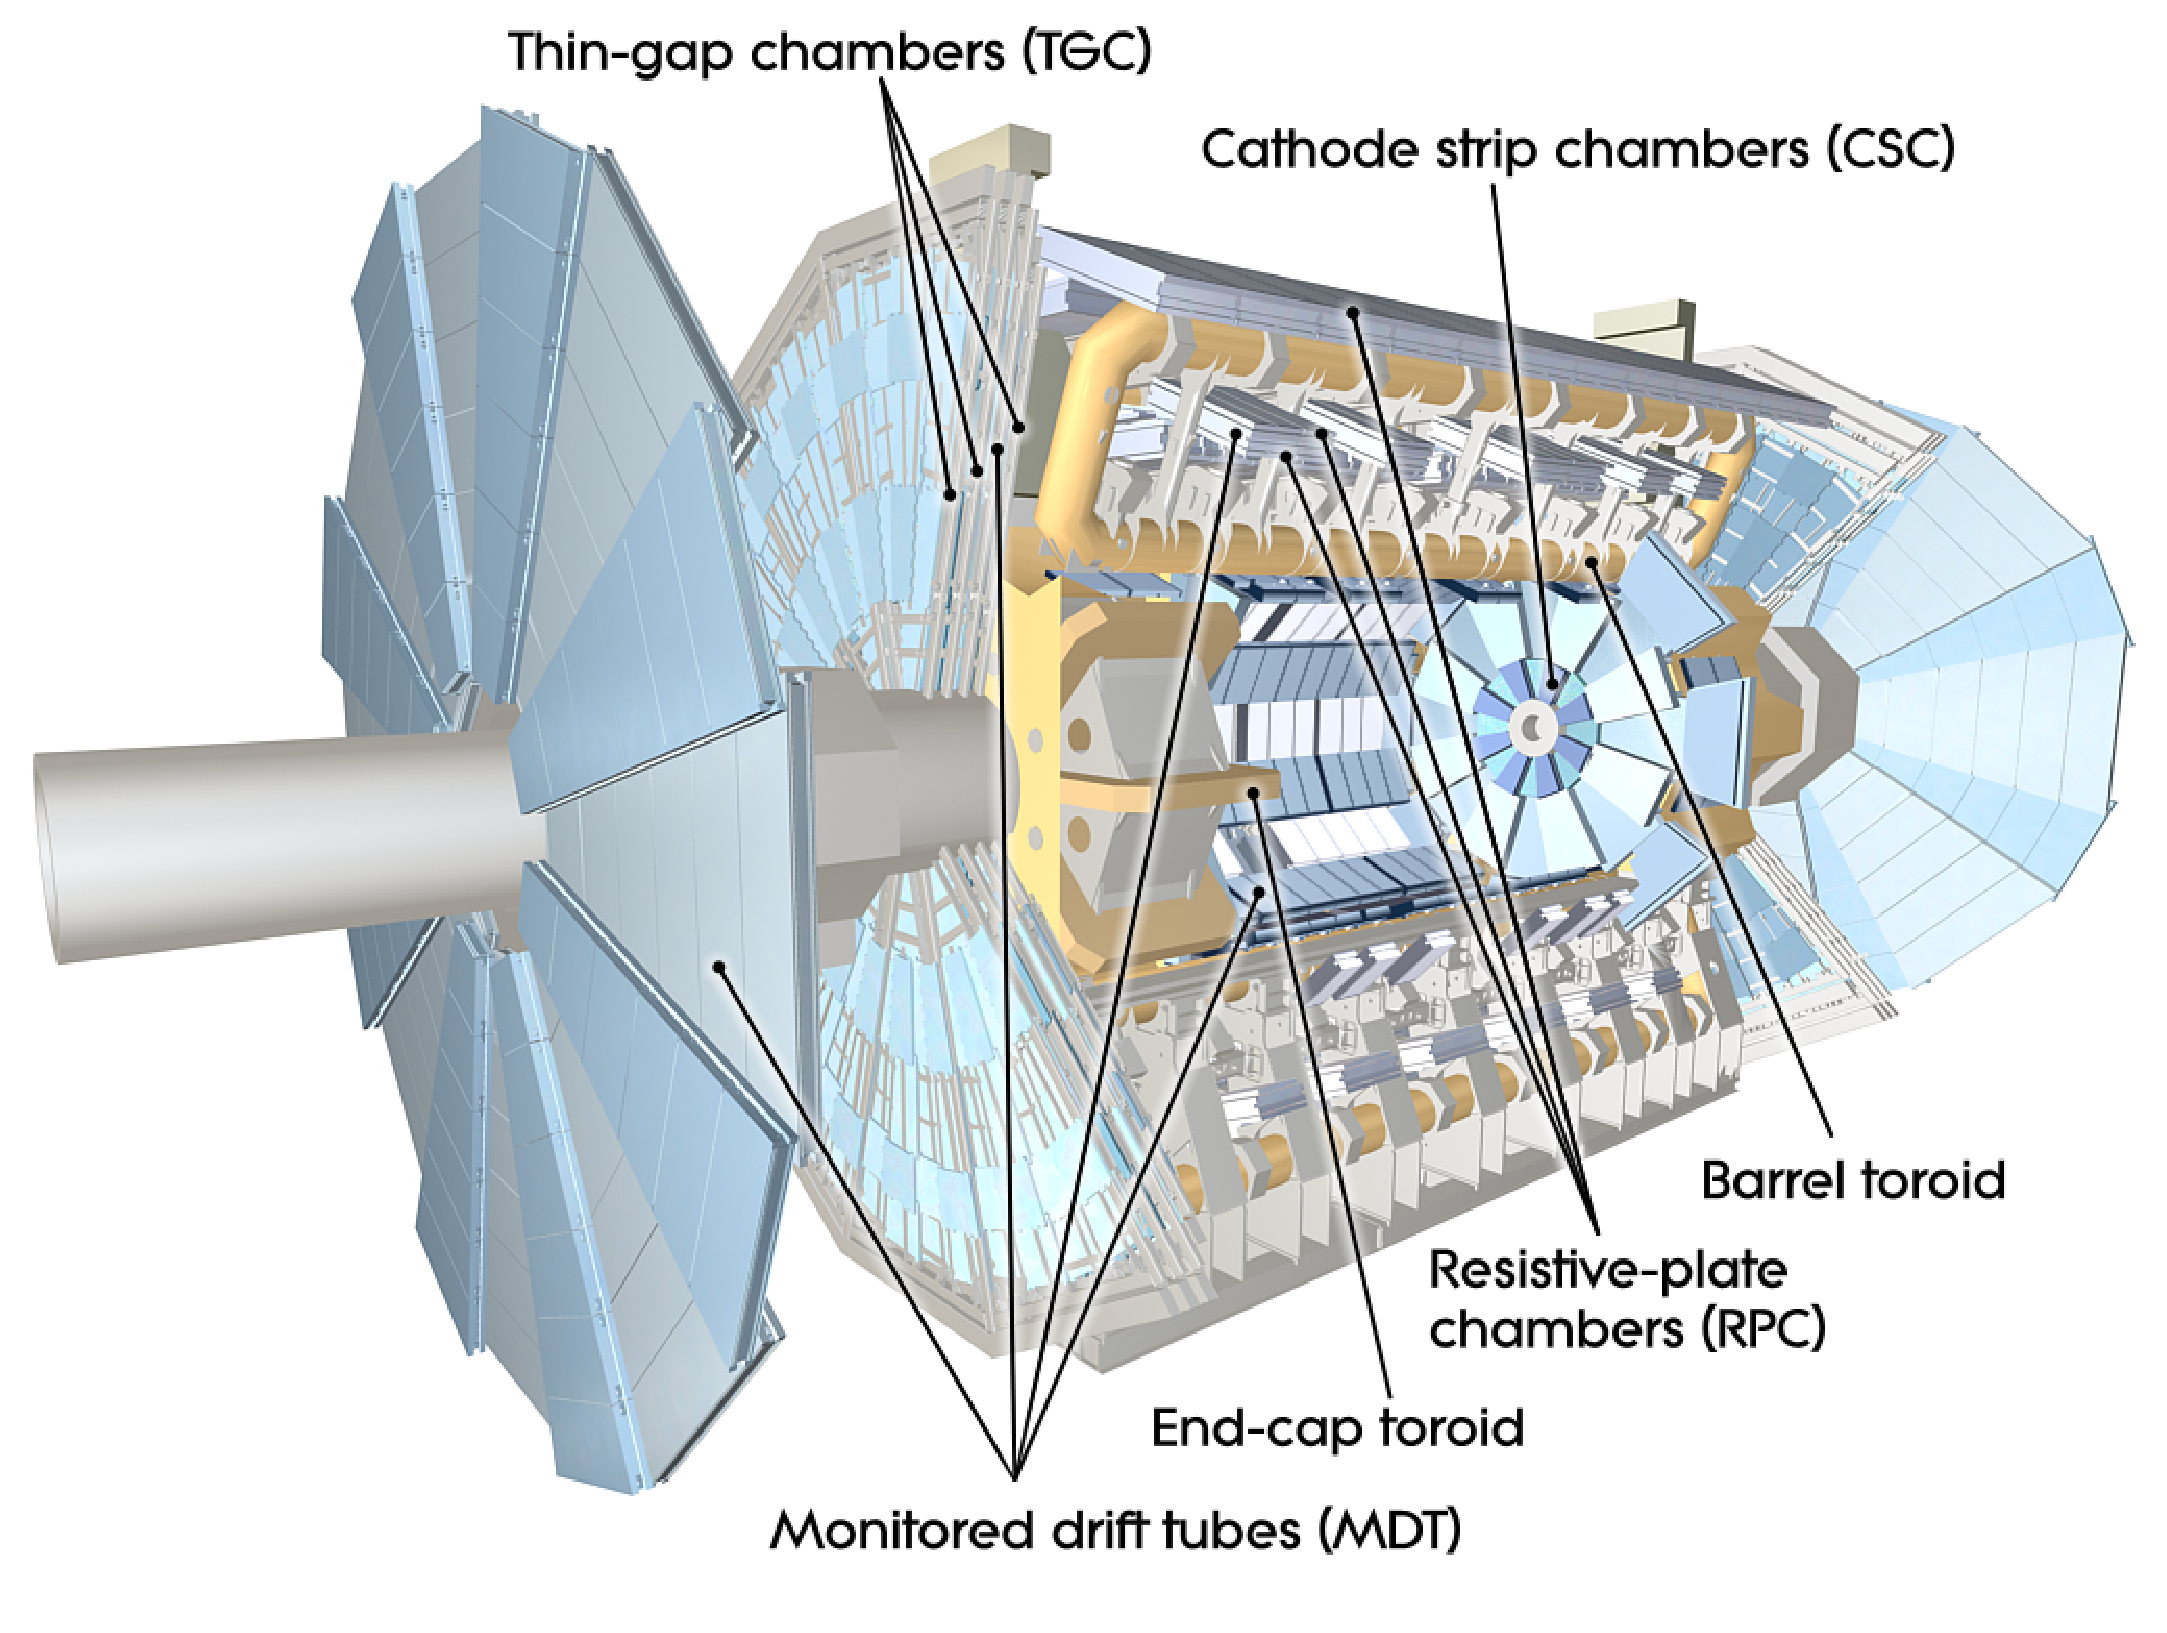
\includegraphics[width=0.80\textwidth]{PartDetector/Diagrams/ATLAS_MuonSystem.eps}
  \caption[Cut-away drawing of the ATLAS muon system.]{Cut-away drawing of the ATLAS muon system~\cite{Detector:ATLASExperimentGeneral}.}
  \label{fig:DetectorDrawingMuonSystem}
\end{figure}

The structure of the MS is delimited by the magnet system. In the barrel region, three cylindrical layers of precision-tracking chambers are located in and on the coils of the barrel toroid magnet at radii of ~\SIlist{5;7.5;10}{\meter}. End-cap region coverage is provided by three chamber planes perpendicular to the $z$-axis. These are located in front and behind the end-cap toroid magnet at distances $|z|\approx$~\SIlist{7.4;10.8;14;21.5}{\meter} from the interaction point.

The MS contains four different types of chambers responsible for precision-tracking and/or triggering in various pseudorapidity ranges, as shown in Table~\ref{tab:DetectorMSOverview}. The arrangement of these chambers is shown in Figure~\ref{fig:DetectorMuonOverview}.

\begin{table}[htb]
  \centering
  \begin{tabular}{@{}ll@{}}
    \toprule
    \textbf{Monitored drift tubes} & \textbf{MDT} \\
    \midrule
    - Coverage                     & $\aeta<2.7$ (innermost layer: $\aeta<2.0$) \\
    - Number of chambers           & 1150 \\
    - Function                     & Precision tracking \\
    \bottomrule
    \textbf{Cathode strip chambers} & \textbf{CSC} \\
    \midrule
    - Coverage                      & $2.0<\aeta<2.7$ \\
    - Number of chambers            & 32 \\
    - Function                      & Precision tracking \\
    \bottomrule
    \textbf{Resistive place chambers} & \textbf{RPC} \\
    \midrule
    - Coverage                        & $\aeta<1.05$ \\
    - Number of chambers              & 606 \\ 
    - Function                        & Triggering, second coordinate \\
    \bottomrule
    \textbf{Thin gap chambers}        & \textbf{TGC} \\
    \midrule
    - Coverage                        & $1.05<\aeta<2.7$~(2.4 for triggering) \\
    - Number of chambers              & 3588 \\
    - Function                        & Triggering, second coordinate \\
    \bottomrule
  \end{tabular}
  \caption[Main parameters of the muon system.]{Main parameters of the muon system~\cite{Detector:ATLASExperimentGeneral}.}
  \label{tab:DetectorMSOverview}
\end{table}

\begin{figure}[tbhp]
  \centering
    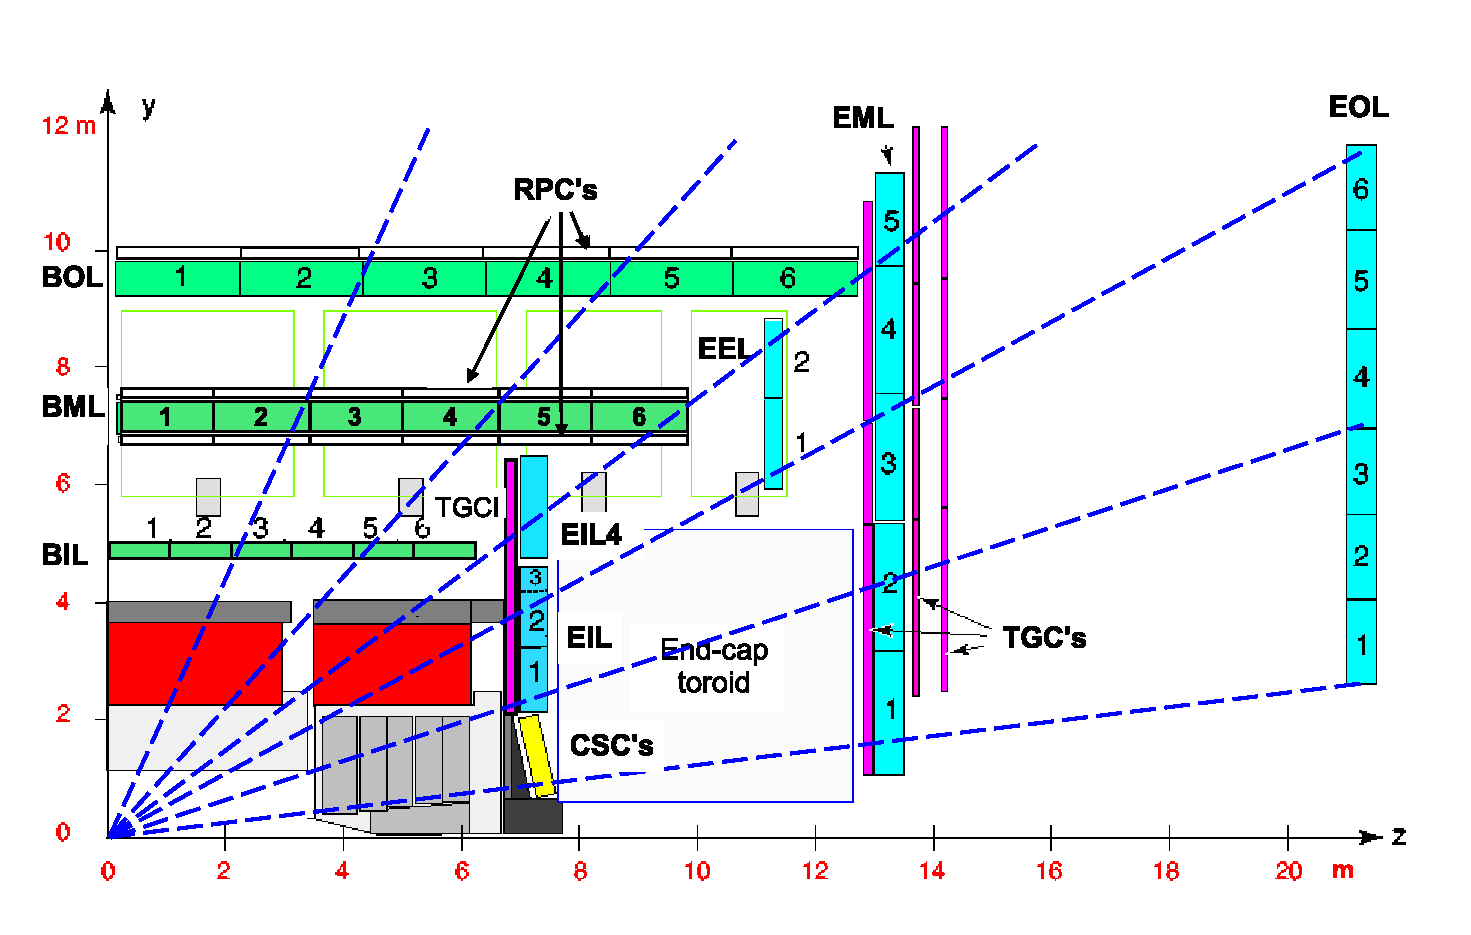
\includegraphics[width=0.80\textwidth]{PartDetector/Diagrams/Muon_section.eps}
    \caption[Plan view of quarter-section of the ATLAS muon spectrometer.]{Plan view of quarter-section of the ATLAS muon spectrometer~\cite{Detector:ATLASExperimentGeneral}.}
  \label{fig:DetectorMuonOverview}
\end{figure}

\begin{figure}[htbp]
  \centering
    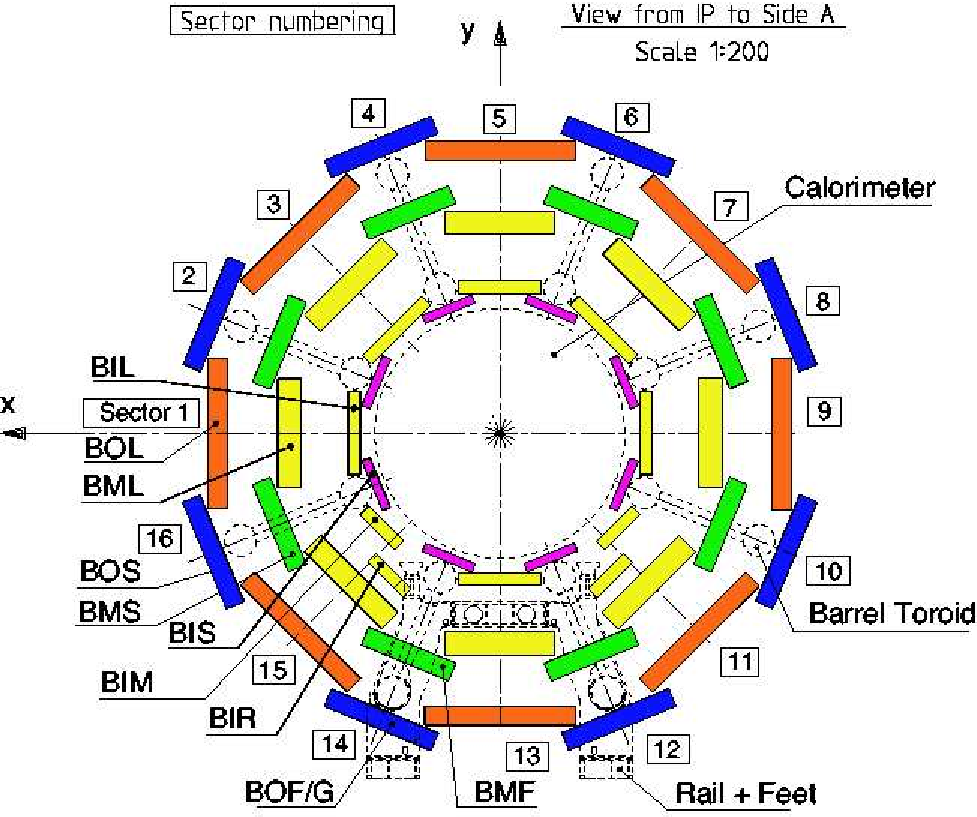
\includegraphics[width=0.80\textwidth]{PartDetector/Diagrams/Muon_sector_numbering.pdf}
    \caption[Transverse view of the muon system.]{Transverse view of the muon system~\cite{Detector:ATLASExperimentGeneral}.}
  \label{fig:DetectorTransverse}
\end{figure}

In the barrel region, precision-measurement is performed by monitored drift tube (MDT) chambers. These chambers consist of three to eight pressurized aluminium drift tubes, each containing a tungsten-rhenium wire anode and a mixture of argon and carbon dioxide gas. An average spatial resolution of \SI{80}{\um} per tube and \SI{35}{\um} per chamber is achieved.

The end-cap region is instrumented with cathode-strip chambers (CSC) due to their higher rate capability and time resolution. CSCs are multi-wire chambers with cathode planes segmented into strips in orthogonal directions, this allows both coordinates to be measured simultaneously. The resolution of a chamber is \SI{40}{\um} in the bending plane ($R$-$z$) and \SI{5}{\mm} in the transverse plane.

Triggering on muon tracks is another essential role of the muon spectrometer. To this end, each precision-measurement chamber is complemented with fast triggering chambers. As with the measurement layers, two different types of chambers are used for the barrel and end-cap regions. In the barrel region ($|\eta<1.05$), resistive plate chambers (RPC) are attached to the same support structure as the MDTs. The RPCs are made of two resistive plates, \SI{2}{\mm} apart, between which a potential difference is applied. The gap between the plates is filled with a mixture of $\textrm{C}_2\textrm{H}_2\textrm{F}_4$/Iso-$\textrm{C}_4\textrm{H}_{10}$/$\textrm{SF}_6$. The signal is read out via metallic strips mounted to the outer faces of the resistive plates. The end-cap region ($1.05<\aeta<2.4$) is populated with thin gap chambers (TGC). TGCs are multi-wire chambers like those used in the CSC, however the distance between the wire and the cathode is smaller in the TGC. A summary of the spatial and temporal resolution for the measurement and triggering layers is shown in Table~\ref{tab:MSPerfomanceSummary}.
%
\begin{table}[htb]
  \centering
  \sisetup{range-phrase=-,range-units=single}
  \begin{tabular}{@{}lccc@{}}
   \toprule
   Chamber & \multicolumn{3}{c}{Resolution in} \\
   \cmidrule{2-4}
           & $R/z$ & $\phi$ & Time \\
   \midrule
   MDT & \SI{35}{\um} $(z)$        & --                  & --            \\
   CSC & \SI{40}{\um} $(R)$        & \SI{5}{\mm}         & \SI{7}{\ns}   \\
   RPC & \SI{10}{\mm} $(z)$        & \SI{10}{\mm}        & \SI{1.5}{\ns} \\ 
   TGC & \SIrange{2}{6}{\mm} $(R)$ & \SIrange{3}{7}{\mm} & \SI{4}{\ns}   \\
   \bottomrule
  \end{tabular}
  \caption[Summary of spatial and temporal resolutions per chamber for all chamber types used in the ATLAS muon spectrometer.]{Summary of spatial and temporal resolutions per chamber for all chamber types used in the ATLAS muon spectrometer. Adapted from~\cite{Detector:ATLASExperimentGeneral}.}
  \label{tab:MSPerfomanceSummary}
\end{table}

\subsection{Magnet system}
The structure of the ATLAS detector is defined by its large magnet systems as shown in Figure~\ref{fig:DetectorMagnet}. The system consists of two sets of magnets: the CS and three air-core toroids.

The CS is located nearest to the beam and provides a \SI{2}{\tesla} magnetic field for the ID for the purpose of tracking, particle identification and \pt\ measurement.

The barrel toroids extend to $\aeta<1.4$ and are made of eight coils, generating a \SI{0.5}{\tesla} magnetic field for the MS. In the high pseudorapidity range, magnetic deflection is provided by two end-cap toroids extending from $1.6<\aeta<2.4$. As in the barrel, the end-cap toroids are made of eight coils offset by \SI{22.5}{\degree} with respect to the barrel coils. Each end-cap generates a \SI{1}{\tesla} magnetic field for the MS. The so-called transition region between the two magnets is covered by the overlap of the end-cap and barrel fields.

\begin{figure}[htbp]
  \centering
  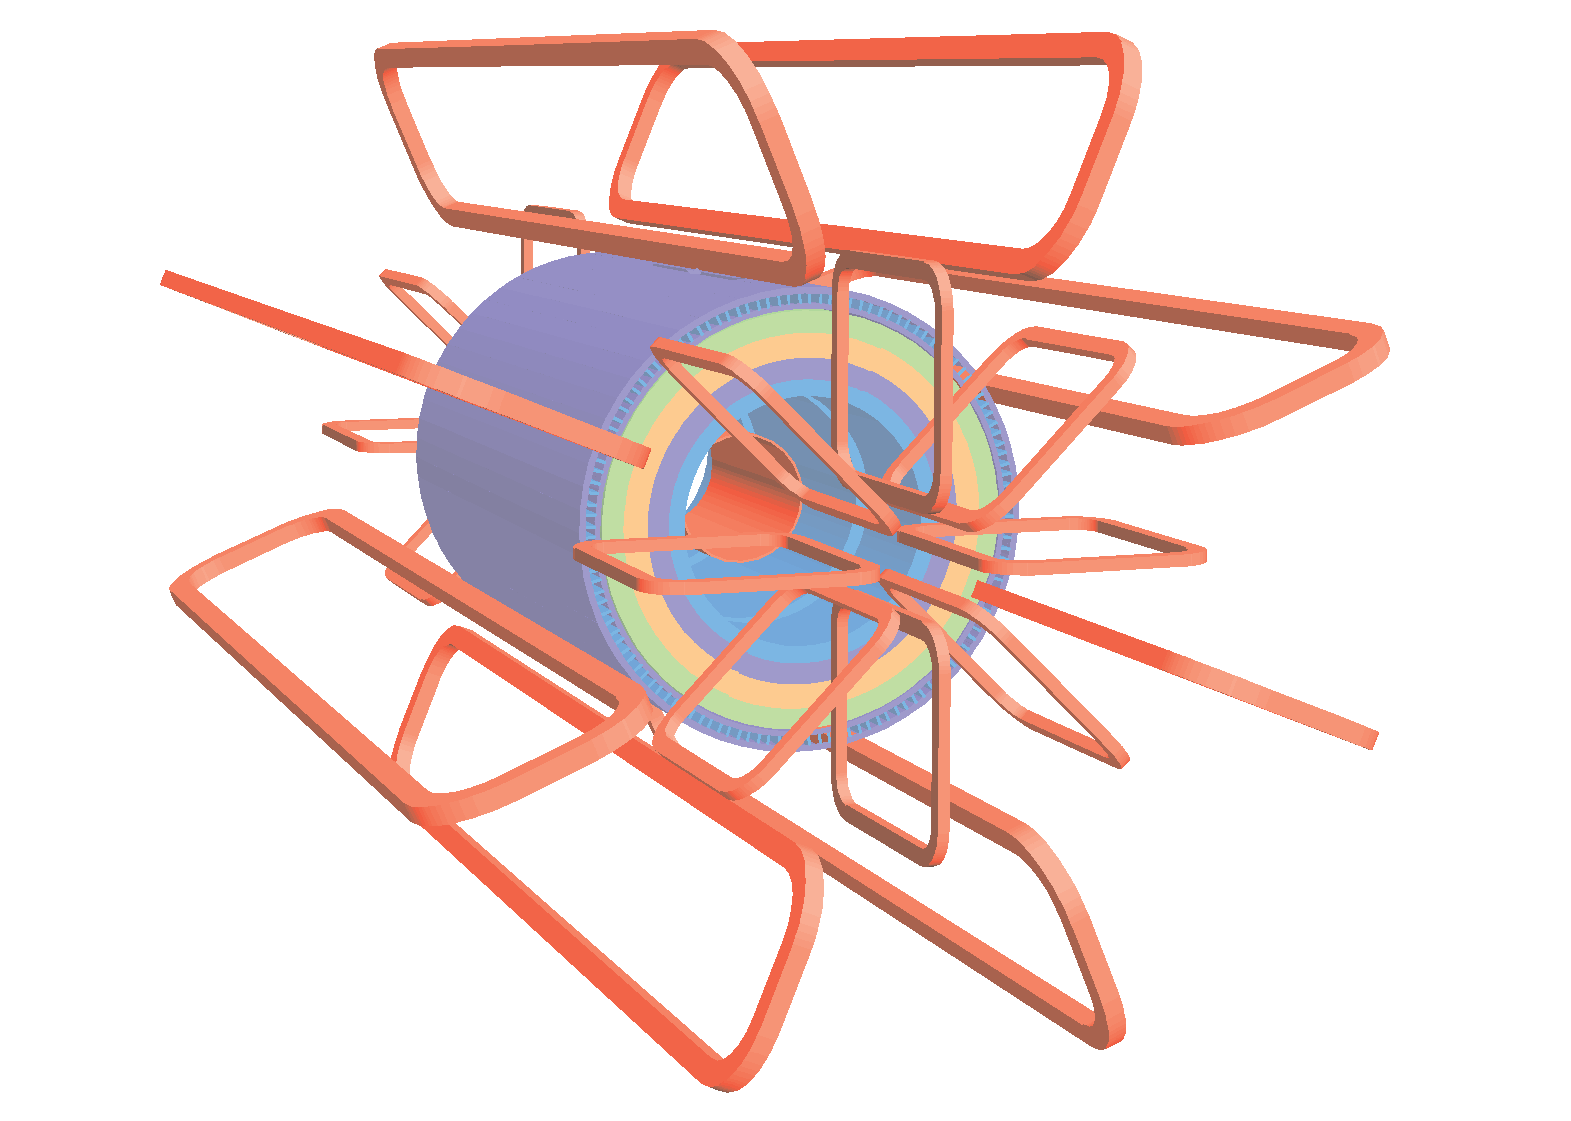
\includegraphics[width=0.80\textwidth]{PartDetector/Diagrams/ATLcoilGeom.eps}
  \caption[Diagram of the ATLAS toroid magnet system.]{Diagram of the ATLAS toroid magnet system~\cite{Detector:ATLASExperimentGeneral}. The red central solenoid is located closest to the beam surrounded by layers of tile calorimetry. The eight barrel toroid magnets are shown along with the offset end-cap toroids at each end.}
  \label{fig:DetectorMagnet}
\end{figure}

\subsection{Beam-pipe}

The beam-pipe section located within the ATLAS experiment is approximately \SI{38}{\meter} in length and made of seven parts. The central chamber has an inner diameter of \SI{58}{\mm} and is constructed from \SI{0.8}{\mm} thick beryllium due to the material's transparency to particles, high specific stiffness and compatibility with ultra-high vacuum. The beam-pipe is centred around the IP and integrated with the pixel detector. The additional layers are made of stainless steel located symmetrically on both sides of the IP.

\subsection{Triggering and data-acquisition}

At the design luminosity of the LHC $\Lagr=\SI{10e34}{\per\square\cm\per\second}$, the expected event rate is approximately \SI{1}{\GHz}. At an average event size of \SI{1.3}{\mega\byte} per event, the total amount of data produced at ATLAS is \SI{1.2}{\peta\byte\per\second}. The maximum rate of data storage at ATLAS is approximately \SI{300}{\mega\byte\per\second}, so the rate must be reduced.

The trigger and data acquisition system (TDAQ) is responsible for reducing the rate by recording only ``interesting'' events. This is known as \emph{online selection} as it happens before the data is stored. In contrast, \emph{offline selection} happens after the data has been recorded, for example when performing a cross section measurement. The overwhelming majority of events produced at the LHC are of no interest to physics analysis. 

At ATLAS, trigger decisions are carried out in three sequential levels: \emph{Level 1} (L1), \emph{Level 2} (L2) and \emph{Event Filter} (EF), each successive level reduces the rate by applying more complex selection criteria. The hardware-based L1 trigger, performs the initial selection based on reduced-granularity information from the MS trigger chambers and all calorimeters. Data from the calorimeter trigger towers, shown in Figure~\ref{fig:DetectorECalSegment}, is used to search for high transverse-momentum muons, photons, electrons, hadronic decays of $\tau$ leptons, hadronic jets, large missing transverse energy, and large total transverse energy. The central trigger processor applies the trigger `menu' which includes a combination of selection criteria. Events which are of interest to physics analyses can be produced at such a rate as to overwhelm the capabilities of the DAQ. A \emph{prescale} can be applied to record one out of many of these events, thus reducing the rate. The L1 trigger also constructs \emph{regions of interest} (RoIs) around the detector where interesting features have been found. The $\eta$ and $\phi$ information of the RoI along with information about the decision is stored and passed to the higher level triggers.

The L2 selection makes use of RoIs and the full granularity of the detector to further reduce the event rate to approximately \SI{3.5}{\kHz}, and finally the EF implements selections commonly used for offline analysis to reduce the rate to \SI{200}{\Hz}.

